\documentclass[11pt]{article}
\usepackage[T1]{fontenc}
\usepackage{lmodern}
\usepackage[margin=1in]{geometry}
\usepackage{amsmath,amssymb,amsthm,mathtools}
\usepackage{graphicx,booktabs,longtable,array,enumitem,xcolor,microtype,xurl}
\usepackage[colorlinks=true,linkcolor=blue!40!black,
 citecolor=blue!40!black,urlcolor=blue!50!black]{hyperref}
\usepackage{bookmark}
\usepackage[section]{placeins}
\emergencystretch=3em
\setcounter{tocdepth}{2}
\numberwithin{equation}{section}
\theoremstyle{plain}
\newtheorem{theorem}{Theorem}[section]
\newtheorem{lemma}[theorem]{Lemma}
\newtheorem{proposition}[theorem]{Proposition}
\newtheorem{corollary}[theorem]{Corollary}
\newtheorem{conjecture}[theorem]{Conjecture}
\theoremstyle{definition}
\newtheorem{definition}[theorem]{Definition}
\theoremstyle{remark}
\newtheorem{remark}[theorem]{Remark}
\newtheorem{example}[theorem]{Example}
\DeclareMathOperator{\Li}{Li}
\DeclareMathOperator{\rank}{rank}
\DeclareMathOperator{\Sym}{Sym}
\DeclareMathOperator{\ad}{ad}
\DeclareMathOperator{\Res}{Res}
\DeclareMathOperator{\Cov}{Cov}
\DeclareMathOperator{\Var}{Var}
\DeclareMathOperator{\Span}{span}
\DeclareMathOperator{\GL}{GL}
\DeclareMathOperator{\SL}{SL}
\newcommand{\Q}{\mathbb Q}
\newcommand{\R}{\mathbb R}
\newcommand{\C}{\mathbb C}
\newcommand{\Z}{\mathbb Z}
\newcommand{\N}{\mathbb N}
\newcommand{\src}[1]{\nolinkurl{#1}}
\newcommand{\sh}{\mathbin{\rotatebox[origin=c]{180}{\ensuremath{\amalg}}}}
\newcommand{\ones}[1]{\{1\}^{#1}}
\newcommand{\wt}{\operatorname{wt}}
\newcommand{\dep}{\operatorname{dep}}
\newcommand{\F}{\mathcal F}
\newcommand{\Lcal}{\mathcal L}
\newcommand{\Ecal}{\mathcal E}
\newcommand{\eps}{\varepsilon}
\title{Polylogarithms: Uniform Bounds and Structural Transitions\\[6pt]
\large Sharp Euler constants, M\"obius depth, radial degeneracies,\\
and a square-root scale for reflected log-gamma coefficients}
\author{A research continuation prepared for Vladimir Reshetnikov\\
\small ProveIt research programme}
\date{10 October 2026}
\hypersetup{pdftitle={Polylogarithms: Uniform Bounds and Structural Transitions},
 pdfauthor={ProveIt research continuation, prepared with OpenAI assistance}}
\begin{document}
\maketitle
\begin{abstract}
We continue the current ProveIt manuscript along four concrete open
directions. First, a sharp two-point inequality for the Euler remainder
kernel proves one-sided enclosures for every real outer order $a\geq0$
and inner order $b>0$. The optimal uniform constant is the previously
identified Gaussian axis maximum
$C_*=\max_{b>0}\{\beta(b)+2^{-b}\eta(b)\}$; the new result is the
remainder comparison that makes this magnitude extremum an error
constant. An exact finite certificate gives $C_*<57/50$. A positive gamma-series
identity yields a moving-order phase law and the asymptotically optimal
global scaled-error constant one, with an explicit lower asymptotic
for its approach.
Second, a binary free-Lie decomposition and confluent interpolation
compute the formal depth reached by any prescribed number of projective
letter directions, including the six M\"obius transformations. Certificates for an established
Nielsen reduction and a corresponding weight-eight obstruction illustrate
the distinction between a formal certificate and a numerical period relation.
Third, rational interval arithmetic isolates a simultaneous quadratic
and quartic radial degeneracy and proves a negative sixth coefficient.
The resulting local families exhibit a quarter-power birth of a maximum
and a region with a minimum followed by a maximum. Finally, a uniform
saddle analysis proves Gaussian damping when the reflected exponent
is of order the square root of the late coefficient index, together
with a growing-exponent half-term truncation law. A shifted saddle
extends the coefficient result to a small proportional range and
resolves a further cubic transition. Proofs, exact
certificates, diagnostic computations, proposed manuscript changes,
and a focused research agenda are supplied. No numerical residual
is promoted to an identity, and no claim of numerical period
independence or global priority is made.
\end{abstract}
\vspace{1em}
\noindent\textbf{Repository baseline.}
\src{3447bc59b78d138a7f0d536b66ac6e5cc5d5e49f}.\\
\textbf{Primary manuscript.}
\src{Analysis/Polylogarithms/docs/manuscript/polylogarithms.tex}.\\
\textbf{Proof status.} Ordinary mathematical proofs and exact finite
arithmetic certificates; no proof-assistant formalization.
\clearpage
{\small\tableofcontents}
\clearpage
\section{Scope, baseline, and the new results}
\label{sec:scope}

The linked repository contains a consolidated manuscript, not merely
the earlier collection of experimental identities. At the pinned
revision it has already incorporated proofs of the Gaussian weight-six
double identities, the displayed weight-four triples, the mixed $S_4$
relation, several rank formulas, and the cubic and quartic
trilogarithm ladders. It also contains sharp real-order kernel theorems,
integral distribution modules, reflected moments, and a substantial
zero-geometry programme. Those advances must be treated as the
starting point. Repeating them would not answer the request for a
continuation.

We audited the active questions against the source chapters and the
later reports preserved beside them. Four directions admit substantive
progress with proofs that can be stated precisely and checked
independently. They share a method: first find the exact object that
controls the question, and then separate its analytic or algebraic
structure from numerical diagnostics. For Euler errors that object is
a two-point kernel difference. For depth it is the osculating span of
binary forms. For radial transitions it is a convergent implicit
equation, together with certified low-order derivatives. For reflected
moments it is a saddle integral with an oscillatory amplitude and a
signed cut representation.

\subsection{A theorem and status ledger}

\begin{longtable}{@{}>{\raggedright\arraybackslash}p{0.18\textwidth}>{\raggedright\arraybackslash}p{0.35\textwidth}>{\raggedright\arraybackslash}p{0.40\textwidth}@{}}
\toprule
Direction & Status in the audited material & Contribution of this article\\
\midrule
\endhead
Euler errors & Order-dependent bounds; sharp critical constant;
axis magnitude maximum; unrestricted remainder comparison open.
& A sharp all-order remainder theorem, its optimal global constant,
an exact rational budget, positive moment identities, and a moving-order
phase law with an asymptotically optimal constant and an explicit
lower asymptotic for its approach.\\[5pt]
Formal depth & Exact calculations, including a weight-six obstruction
and special transformations.
& An all-weight formula for any number of projective directions;
six-map versus full-linear comparison; exact certificates for known
Nielsen reductions, with literature attribution.\\[5pt]
Radial geometry & Both signs of the quartic coefficient on the quadratic
threshold; a diagnostic simultaneous zero.
& Exact isolation, negative sixth coefficient, a quarter-power law,
a two-extremum local unfolding, and a fully explicit rational example.\\[5pt]
Reflected coefficients & Fixed reflected exponent asymptotics and
fixed-exponent optimal truncation.
& A uniform $m=O(\sqrt{k})$ transition, Gaussian damping, explicit
first correction, a growing-exponent half-term law, and a small proportional saddle theorem.\\[5pt]
Special-value candidates & $S_6$ and the revised $S_8$ candidate remain
conjectural despite certified small residuals.
& Their evaluation status is unchanged; the new formal obstruction
specifies a limitation of a particular reduction method.\\
\bottomrule
\end{longtable}
\addtocounter{table}{-1}

The labels ``new'' and ``open'' in this article refer to the audited
repository state. The general tools---Euler transformation, gamma
integrals, free-Lie character theory, Hermite interpolation, analytic
implicit inversion, and the saddle method---are classical. We do not
claim that a broad literature search could establish priority for every
consequence. The article supplies proofs of the stated refinements
and records the primary sources used for their background.

\subsection{Conventions and the interpretation of identities}

Multiple polylogarithms use decreasing nested indices:
\[
 \Li_{s_1,\ldots,s_d}(z_1,\ldots,z_d)
 =\sum_{n_1>\cdots>n_d\geq1}
        \frac{z_1^{n_1}\cdots z_d^{n_d}}
             {n_1^{s_1}\cdots n_d^{s_d}}
\]
where the series converges. A one-variable specialization means
$\Li_{s_1,\ldots,s_d}(z,1,\ldots,1)$. Real-order $F_{a,b}$ is
defined explicitly in Section~\ref{sec:euler}, so no convention for
nonintegral-depth words is needed. All analytic continuations use the
principal branch unless a simply connected path domain is specified.
Statements at $i$ concern analytic or Abel values where the ordinary
Fourier series fails to converge.

Formal identities in a shuffle quotient have a different meaning.
Their vanishing proves an exact congruence modulo the stated product
and endpoint-constant relations. A nonzero class proves the absence
of a certificate using those relations. It does not prove numerical
independence of periods and does not exclude other functional
equations. Section~\ref{gorbit:sec:main} gives the exact comparison space
before drawing any depth conclusion.

For parameter estimates, terminating decimal endpoints are rational
numbers. They can therefore be part of a finite exact proof when
every operation is outward rounded and every transcendental input
has a proved remainder bound. By contrast, a printed approximate
root or a many-digit agreement from quadrature is diagnostic unless
an enclosure theorem is also supplied.

\subsection{What is reproducible}

The archive includes this source and its compiled PDF, independent
exact verifiers for the finite claims, numerical checks that compare
different representations, and the resulting machine-readable data.
The new statements are proved in the text; the code has three
different roles, explicitly separated in the verification section:
finite arithmetic proof certificates, finite corroboration of a
general algebraic theorem, and nonrigorous asymptotic diagnostics.

The repository was read at the pinned revision without applying
changes to it. Suggested chapter insertions and wording replacements
are supplied separately. The package can thus be reviewed and
integrated against a concrete baseline without silently altering
historical reports or their recorded status.

\section{A sharp uniform Euler bound at every positive real order}
\label{sec:euler}

The canonical manuscript proves one-sided Euler enclosures in several
parameter regions. It also proves that the Gaussian magnitude has a unique
global maximum on the outer-order axis. It explicitly cautions that a
magnitude bound alone is not a remainder bound in the supercritical
region. The missing implication is supplied here by a sharp, elementary
two-point inequality. No finite signed-moment representation is needed.

\subsection{Definitions and the exact two-measure representation}

For $a\geq0$, $b>0$, let
\[
 H_m^{(b)}=\sum_{j=1}^m j^{-b},\qquad
 F_{a,b}(z)=\sum_{n\geq1}\frac{H_{n-1}^{(b)}}{n^a}z^n,
 \qquad |z|<1.
\]
For integral positive orders this is the decreasing-index multiple
polylogarithm $\Li_{a,b}(z,1)$. Write
$g_{a,b}=\Im F_{a,b}(i)$ for the principal analytic value, and set
\begin{equation}\label{eq:euler-defs}
 f_n=\frac{H_{2n}^{(b)}}{(2n+1)^a},\quad
 d_j=\sum_{n=0}^j(-1)^n\binom jn f_n,\quad
 E_N=\sum_{j=0}^{N-1}\frac{d_j}{2^{j+1}}\quad(N\geq1).
\end{equation}
Thus $f_0=d_0=E_1=0$. The sign convention for $d_j$ is $(-1)^j$
times the usual forward difference. Euler's classical transformation
is recalled in DLMF~\cite{DLMFEuler}; our task is to prove its continuation,
sign, and sharp uniform error throughout the present real-order family.

For $s>0$, define a probability measure on $(0,1)$ by
\[
 d\sigma_s(t)=\frac{(-\log t)^{s-1}}{\Gamma(s)}\,dt,
 \qquad \sigma_0=\delta_1.
\]
Its moments are $\int_0^1t^{n-1}\,d\sigma_s(t)=n^{-s}$.
Writing the inner harmonic number as a geometric sum gives
\begin{equation}\label{eq:two-moment}
 \frac{H_{n-1}^{(b)}}{n^a}
 =\iint t^{n-1}\frac{1-u^{n-1}}{1-u}\,
                       d\sigma_a(t)d\sigma_b(u).
\end{equation}
This includes $n=1$, when the integrand is zero. For every fixed $n$
it is bounded, so no cancellation of divergent integrals is involved.

\begin{lemma}[Two-measure continuation]\label{lem:two-measure}
For $a\geq0$, $b>0$, the identity
\begin{equation}\label{eq:F-double}
 F_{a,b}(z)=z^2\iint
        \frac{t}{(1-tz)(1-tuz)}\,d\sigma_a(t)d\sigma_b(u)
\end{equation}
holds on $\mathbb C\setminus[1,\infty)$. In particular,
\begin{equation}\label{eq:g-double}
 -g_{a,b}=\iint\frac{t^2(1+u)}{(1+t^2)(1+t^2u^2)}
                           \,d\sigma_a(t)d\sigma_b(u)>0.
\end{equation}
For $j\geq1$,
\begin{equation}\label{eq:d-double}
 d_j=-\iint\frac{(1-t^2u^2)^j-(1-t^2)^j}{1-u}
                           \,d\sigma_a(t)d\sigma_b(u)<0.
\end{equation}
\end{lemma}
\begin{proof}
Insert \eqref{eq:two-moment} in the disk series and sum the two
geometric series. Absolute convergence on compact subdisks justifies
the interchange. On a compact subset of the slit plane, both denominators
in \eqref{eq:F-double} are bounded away from zero uniformly for
$t,u\in[0,1]$. The integral is therefore holomorphic there and gives
the asserted continuation. Rationalizing at $i$ proves
\eqref{eq:g-double}. Applying the finite binomial theorem to
\eqref{eq:two-moment} proves \eqref{eq:d-double}. The numerator is
strictly positive for $t>0$, $0<u<1$, giving the sign.
\end{proof}

\subsection{The sharp two-point kernel inequality}

Put
\[
 W_N(x)=\frac{(1-x)^N}{1+x},\qquad 0\leq x\leq1.
\]
The two arguments of $W_N$ will be $t^2u^2$ and $t^2$.

\begin{lemma}[Power-difference maximum]\label{lem:power-difference}
Let $0<v<1$ and let $k\geq2$ be an integer. Then
\begin{align}\label{eq:power-max}
 \max_{0\leq x\leq1}\{(1-vx)^k-(1-x)^k\}
 &=\frac{(1-v)^k}{(1-v^{k/(k-1)})^{k-1}}\\[-2pt]
 &\leq\frac{1-v}{1+v}.\notag
\end{align}
The second inequality is an equality when $k=2$, and is strict when
$k>2$.
\end{lemma}
\begin{proof}
Differentiation shows that the unique interior maximizer satisfies
$(1-x)/(1-vx)=v^{1/(k-1)}$. Substitution gives the displayed maximum.
For $1\leq p\leq2$, the function
\[
 H(p)=\log(1-v^p)-\log(1-v)-(p-1)\log(1+v)
\]
has $H(1)=H(2)=0$ and
\[
 H''(p)=-\frac{v^p(\log v)^2}{(1-v^p)^2}<0.
\]
Thus $1-v^p\geq(1-v)(1+v)^{p-1}$, with strict inequality
for $1<p<2$. Take $p=k/(k-1)$ and raise to the power $k-1$.
\end{proof}

\begin{theorem}[Sharp Euler kernel modulus]\label{thm:kernel}
For $N\geq1$, $0\leq x\leq1$, and $0<v<1$,
\begin{equation}\label{eq:kernel-bound}
 0\leq W_N(vx)-W_N(x)\leq\frac{1-v}{1+v}.
\end{equation}
The upper bound is attained exactly when $N=1$ and $x=1$.
For $N\geq2$ it is strict for every $x$.
\end{theorem}
\begin{proof}
The nonnegativity follows from the decrease of $W_N$. For $N=1$,
\[
 W_1(vx)-W_1(x)=\frac{2x(1-v)}{(1+x)(1+vx)}.
\]
The comparison with $(1-v)/(1+v)$ is equivalent to
$(1-x)(1-vx)\geq0$, with equality only at $x=1$.
For $N\geq2$, the uniformly convergent geometric expansion
\begin{equation}\label{eq:W-mixture}
 W_N(x)=\sum_{k=N}^{\infty}2^{N-k-1}(1-x)^k
\end{equation}
expresses $W_N$ as a probability mixture of powers. Apply
Lemma~\ref{lem:power-difference} term by term. At least one index
$k>2$ has positive mixture weight, so the upper inequality is strict.
\end{proof}

This proof also explains why a direct estimate by a signed measure's
total variation can be wasteful: the relevant object is a difference
of two values of the remainder kernel, and this difference has a
uniform modulus even where a precursor measure has infinite mass.

\subsection{Uniform continuation and the least possible constant}

Let $\beta(s)=\sum_{n\geq0}(-1)^n/(2n+1)^s$ and
$\eta(s)=\sum_{n\geq1}(-1)^{n-1}/n^s$ for $s>0$, and define
\begin{equation}\label{eq:Cb}
 C(b)=\beta(b)+2^{-b}\eta(b)
     =\int_0^1\frac{1+u}{1+u^2}\,d\sigma_b(u).
\end{equation}
The equality follows either from the residue classes in $\Li_b(i)$
or from \eqref{eq:g-double} at $a=0$. The measure integral also
avoids any question about conditional termwise summation.

\begin{theorem}[All-order Euler enclosure]\label{thm:Euler-uniform}
For every $a\geq0$, $b>0$, the finite sums $E_N$ decrease strictly to
$g_{a,b}$, with
\begin{equation}\label{eq:Euler-exact}
 R_N(a,b):=2^N(E_N-g_{a,b})
 =\iint\frac{W_N(t^2u^2)-W_N(t^2)}{1-u}\,
                       d\sigma_a(t)d\sigma_b(u).
\end{equation}
For all $N\geq1$,
\begin{equation}\label{eq:Euler-b-bound}
 0<R_N(a,b)\leq C(b)<\frac{1+\sqrt2}{2}<\frac54.
\end{equation}
Equality $R_N(a,b)=C(b)$ holds exactly when $a=0$ and $N=1$.
Consequently, for each fixed $b>0$, $C(b)$ is the least error
constant uniform in $a>0$ and $N\geq1$. Furthermore,
$R_N(a,b)\to0$ for every fixed pair.
\end{theorem}
\begin{proof}
For fixed $t,u$, summing the finite geometric series in
\eqref{eq:d-double} and comparing with \eqref{eq:g-double} gives
\eqref{eq:Euler-exact}. All finite integrals exist: a difference
quotient at $u=1$ has a finite continuous limit. Alternatively, the
bound below gives direct domination of the remainder. Apply
Theorem~\ref{thm:kernel} with $v=u^2$, $x=t^2$ and divide by $1-u$:
\[
 0\leq\frac{W_N(t^2u^2)-W_N(t^2)}{1-u}
       \leq\frac{1+u}{1+u^2}.
\]
Integration proves the bound and the equality conditions, since
$\sigma_b$ has positive density on $(0,1)$ and $\sigma_a$ does too
when $a>0$. The maximum of $(1+u)/(1+u^2)$ occurs at
$u=\sqrt2-1$ and equals $(1+\sqrt2)/2$; positivity of the density
makes the corresponding integral inequality strict.
The strict decrease of $E_N$ follows from $d_N<0$. The bound proves
convergence to the analytic value even if the original boundary series
diverges. Finally the integrand tends to zero at every $t,u>0$ with
$u<1$, so dominated convergence gives $R_N\to0$.

For sharpness at fixed $b$, let $a\downarrow0$. If
$T_a\sim\mathrm{Gamma}(a,1)$, then $\mathbb E T_a=a$, so
$e^{-T_a}\to1$ in probability. Thus $\sigma_a\Rightarrow\delta_1$.
At $N=1$, dominated convergence gives $R_1(a,b)\to C(b)$.
No smaller constant can hold uniformly over positive $a$.
\end{proof}

\begin{corollary}[Sharp global constant]\label{cor:Euler-global}
Let $b_*$ denote the unique maximizer of $C$ on $(0,\infty)$, and set
\begin{equation}\label{eq:Cstar}
 C_*=C(b_*)=\max_{b>0}\{\beta(b)+2^{-b}\eta(b)\}.
\end{equation}
Then the sharp uniform strict enclosure for $a,b>0$ is
\begin{equation}\label{eq:sharp-global}
 \boxed{\quad E_N-C_*2^{-N}<g_{a,b}<E_N\quad(N\geq1).\quad}
\end{equation}
It is sharp also over the entire nonnegative outer-order domain, where
the non-strict lower enclosure is attained only at $(a,b,N)=(0,b_*,1)$.
The exact bounds from the manuscript are
\[
 1<b_*<2,\qquad \frac{227}{200}<C_*<\frac{1+\sqrt2}{2}.
\]
The diagnostic numerical values are
\[
 b_*=1.30221658710124120959\ldots,\qquad
 C_*=1.13656110333950956095\ldots.
\]
\end{corollary}
\begin{proof}
The axis maximum, its uniqueness and its nondegeneracy are proved in
the pinned manuscript, \src{05-subcritical-stieltjes.tex},
Theorem~\texttt{subpick:thm:axis-maximum}~\cite{ProveItSnapshot}.
For clarity, the mechanism is that $C(b)=\mathbb E[\phi(T_b)]$,
where $\phi(T)=(1+e^{-T})/(1+e^{-2T})$ has exactly one maximum.
The strict two-intersection property of the Mellin family proves
uniqueness; this is stronger than a numerical root scan.
The new inequality \eqref{eq:Euler-b-bound} supplies the missing
remainder comparison. Maximizing it over $b$ gives the claimed bound.
Its sharpness follows from $N=1$, $b=b_*$, and $a\downarrow0$.
\end{proof}

\begin{figure}[tbp]
\centering
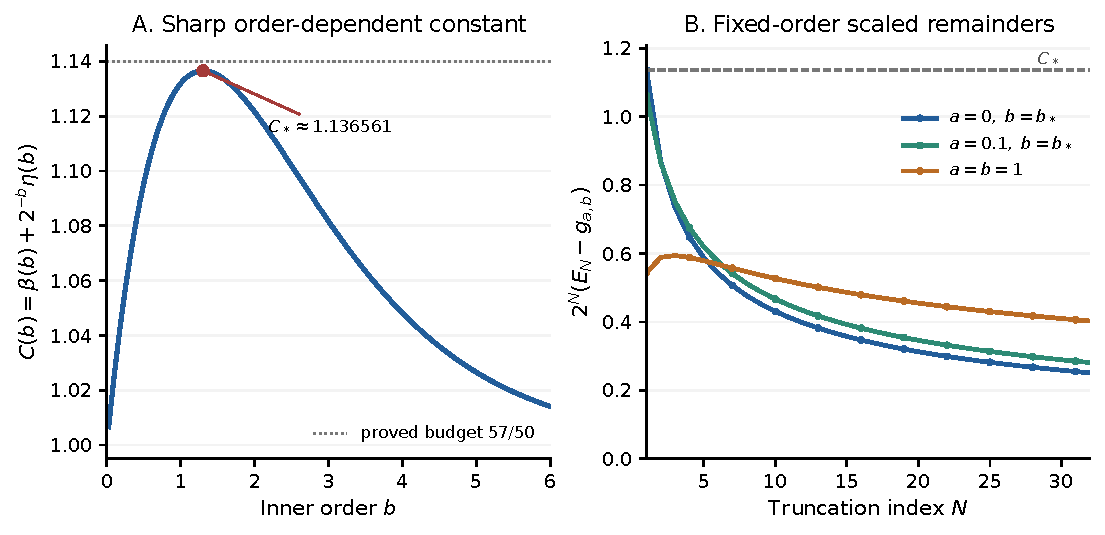
\includegraphics[width=\textwidth]{figures/euler_bounds.pdf}
\caption{Numerical illustrations of the proved Euler bounds.
Panel A shows $C(b)$, its maximum, and the rational budget $57/50$.
Panel B shows fixed-order scaled remainders, including the increase
from $N=1$ to $N=2$ at $a=b=1$. The curve at $a=0$ is the boundary
case allowed by the theorem. The plots illustrate the analytic
proof; the rational global budget is certified separately.}
\label{fig:euler-bounds}
\end{figure}

The constant is specified exactly by \eqref{eq:Cstar}; the decimal
display is not an asserted closed form or a certified enclosure.
The elementary rational constant $5/4$ already follows from the
analytic proof. The following small exact computation improves the
operational constant uniformly over all orders.

\begin{proposition}[A simple rational global budget]\label{prop:rational-budget}
The exact inequalities
\[
 C_*<\frac{5129}{4500}<\frac{57}{50}
\]
hold. Thus $57/50$ is a valid uniform Euler error budget for every
$a\geq0$, $b>0$, and $N\geq1$.
\end{proposition}
\begin{proof}
For $1\leq b\leq2$, gamma differentiation and Cauchy--Schwarz give
\[
 |C'(b)|=|\operatorname{Cov}(\log T_b,\phi(T_b))|
 \leq\sqrt{\psi_1(b)}\,\sqrt{\operatorname{Var}\phi(T_b)}<\frac16.
\]
Indeed $1\leq\phi\leq(1+\sqrt2)/2$ has range less than $1/4$,
so its standard deviation is less than $1/8$. The variance identity
$\operatorname{Var}\log T_b=\psi_1(b)$ follows by differentiating
the gamma integral. Also $\psi_1(b)\leq\psi_1(1)=\pi^2/6<16/9$;
the last inequality follows, for example, from $\pi<22/7$.

The standard-library verifier encloses $C(1+j/30)$ for all
$0\leq j\leq30$ by \eqref{eq:finite-E} with $a=0$, $N=48$,
using a $10^{45}$ grid and integer root inequalities. The already
proved $5/4$ tail bound makes these genuine analytic enclosures.
All thirty-one upper endpoints are strictly less than $1137/1000$.
Every point of $[1,2]$ is within $1/60$ of a node, whence
\[
 C(b)<\frac{1137}{1000}+\frac1{360}=\frac{5129}{4500}
       <\frac{57}{50}.
\]
The proved location $1<b_*<2$ completes the global argument.
Every finite comparison is recorded as a rational inequality in
\src{data/euler_exact_certificate.json}. Neither floating-point
root finding nor a numerical derivative bound enters this proof.
\end{proof}

\begin{remark}[Why the new kernel step is necessary]
At $(a,b)=(1,1)$, the identity
$F_{1,1}(z)=\tfrac12\log^2(1-z)$ gives
$g_{1,1}=-\pi\log2/8$. Therefore
\[
 R_1=\frac{\pi\log2}{4},\qquad
 R_2=\frac{\pi\log2}{2}-\frac12>R_1.
\]
Indeed $\pi>3$ and $\log2>2/3$ imply $\pi\log2>2$.
Thus the scaled errors need not decrease outside the previously
proved right-endpoint region. Bounding $R_N$ by its $N=1$ value
would be invalid even at this simplest integral-order pair.
\end{remark}

\subsection{A general theorem for harmonic sums built from moments}

The argument proves a more general statement that can be reused for
other completely monotone inner sequences. Let $\alpha,\beta$ be
finite positive measures on $[0,1]$, and define
\[
 c_n=\iint t^{n-1}(1+u+\cdots+u^{n-2})\,d\alpha(t)d\beta(u),
 \qquad c_1=0.
\]
Use the definitions \eqref{eq:euler-defs} with $f_n=c_{2n+1}$,
and let $g$ be the imaginary value at $i$ of the continuation
\eqref{eq:F-double}. Difference quotients at $u=1$ are understood
by continuity.

\begin{theorem}[Moment-product Euler principle]\label{thm:moment-general}
For every such pair of measures and every $N\geq1$,
\begin{equation}\label{eq:moment-general}
 0\leq2^N(E_N-g)
 \leq\alpha([0,1])\int_0^1\frac{1+u}{1+u^2}\,d\beta(u)
 \leq\frac{1+\sqrt2}{2}\alpha([0,1])\beta([0,1]).
\end{equation}
The last universal constant is optimal. For probability measures it
is attained at $N=1$, $\alpha=\delta_1$,
$\beta=\delta_{\sqrt2-1}$.
\end{theorem}
\begin{proof}
The finite identities and kernel comparison above remain valid for
arbitrary positive measures. Passing to $u=1$ preserves the inequality
by continuity. The endpoint $t=0$ contributes zero, so it causes no
difficulty. Integrate the pointwise bound, then optimize its last
factor on $[0,1]$. The stated two Dirac masses attain it.
\end{proof}

This theorem identifies the property required for an extension:
the coefficients must be a product of a Hausdorff moment and a finite
partial sum of another moment sequence. It does not assert the same
bound for an arbitrary alternating series or for signed input measures.

\subsection{A certified algorithm and exact identity family}

For every $a\geq0$, $b>0$, the following absolutely convergent identity
is now valid even when the untransformed Gaussian boundary series
fails the term test:
\begin{equation}\label{eq:Euler-identity}
 g_{a,b}=\sum_{j=1}^{\infty}\frac1{2^{j+1}}
       \sum_{n=1}^j(-1)^n\binom jn
           \frac{H_{2n}^{(b)}}{(2n+1)^a}.
\end{equation}
The terms of the outer series are strictly negative, and the first
$N-1$ terms have error bounded by $C(b)2^{-N}$. This is a
proved identity family with an explicit error theorem, rather than
a new name for a formal divergent rearrangement.

The already available finite binomial-tail formula is
\begin{equation}\label{eq:finite-E}
 E_N=2^{-N}\sum_{n=0}^{N-1}(-1)^n
       \frac{H_{2n}^{(b)}}{(2n+1)^a}
                  \sum_{j=n+1}^N\binom Nj.
\end{equation}
The new theorem and Proposition~\ref{prop:rational-budget} supply the
order-independent tail budget $(57/50)2^{-N}$. For rational $a,b$, fractional powers in this finite
sum can be enclosed by integer root inequalities; additions and
multiplications then use rational interval arithmetic. This avoids
the parameter-dependent singular budgets near $a+b=1$ in the earlier
implementation. Given a target absolute radius $\varepsilon$, any
$N$ satisfying $(57/50)2^{-N}\leq\varepsilon$ suffices for the analytic
tail, in addition to the separately controlled finite-sum rounding.

The accompanying program checks this statement using exact rational
arithmetic, including deliberately corrupted candidate controls.
Its numerical comparisons use different representations for selected
known values; a finite check corroborates the analytic proof but does
not replace it. The new global theorem should supplement the more
specialized and sometimes sharper bounds already present in the book.

\subsection{A positive gamma-series identity for the scaled remainder}

The same representation gives an exact identity that exposes the
effect of a large inner order. Let $T,V$ be independent gamma
variables of rate one and respective shapes $a,b$; for $a=0$
take $T=0$ deterministically. Define
\[
 J_N(s)=\mathbb E\bigl[W_N(e^{-2Y_s})\bigr],
 \qquad Y_s\sim\operatorname{Gamma}(s,1),
 \qquad J_N(0)=W_N(1)=0.
\]
In particular, for $s>0$ this is the positive integral
\[
 J_N(s)=\frac1{\Gamma(s)}
 \int_0^\infty y^{s-1}e^{-y}
             \frac{(1-e^{-2y})^N}{1+e^{-2y}}\,dy.
\]

\begin{proposition}[Positive gamma-series identity]
\label{prop:gamma-remainder-series}
For all $a\geq0$, $b>0$ and integers $N\geq1$,
\begin{equation}\label{eq:gamma-remainder-series}
 R_N(a,b)=\sum_{r=1}^{\infty}r^{-b}
  \mathbb E\left[
   W_N\bigl(e^{-2(T+V/r)}\bigr)-W_N(e^{-2T})\right].
\end{equation}
Every summand is nonnegative, and the series converges.
If $b>1$, its first term gives the uniform enclosure
\begin{equation}\label{eq:gamma-remainder-first}
 0\le R_N(a,b)-\{J_N(a+b)-J_N(a)\}\le\zeta(b)-1.
\end{equation}
\end{proposition}
\begin{proof}
In logarithmic coordinates the exact two-measure formula reads
\[
 R_N(a,b)=\mathbb E
 \frac{W_N(e^{-2(T+U)})-W_N(e^{-2T})}{1-e^{-U}},
 \qquad U\sim\operatorname{Gamma}(b,1),
\]
with $T,U$ independent. Expand $(1-e^{-U})^{-1}$ as a
positive geometric series. Tonelli's theorem applies because
the numerator is nonnegative. Multiplying the rate-one gamma
density of $U$ by $e^{-(r-1)U}$ produces $r^{-b}$ times
the density of $V/r$. This proves
\eqref{eq:gamma-remainder-series}; its convergence follows
from Theorem~\ref{thm:Euler-uniform}.
The sum of independent rate-one gamma variables has the
sum of their shapes, so the $r=1$ term is
$J_N(a+b)-J_N(a)$. Every other expectation lies in $[0,1]$,
which proves \eqref{eq:gamma-remainder-first}.
\end{proof}

The enclosure is independent of $a$ and $N$. For large $b$,
it replaces a two-variable integral by a difference of two
positive one-variable integrals with an exponentially small
budget in $b$. For $b\leq1$ the positive series identity
still holds, but the crude tail estimate by $\zeta(b)-1$
must not be used.

\subsection{Logarithmically growing orders: a phase law for Euler errors}

The fixed-order statement $R_N\to0$ cannot be made uniform
over all positive orders. The following theorem identifies
an explicit transition and its two boundary profiles.
Write
\[
 \Phi_{\mathrm G}(x)=\frac1{\sqrt{2\pi}}
                    \int_{-\infty}^x e^{-y^2/2}\,dy
\]
for the standard normal distribution function.

\begin{theorem}[Moving-order Euler phase law]
\label{thm:euler-moving}
Let $\ell=\log N$. Suppose
\[
 a_N=A\ell+\alpha\sqrt{\ell}+o(\sqrt{\ell}),\qquad
 b_N=B\ell+\beta\sqrt{\ell}+o(\sqrt{\ell}),
 \qquad A,B>0,
\]
where $\alpha,\beta$ are fixed real numbers. Then
\begin{equation}\label{eq:euler-phase}
 R_N(a_N,b_N)\longrightarrow
 \begin{cases}
  0,& A+B<1/2,\\
  \Phi_{\mathrm G}(\sqrt2(\alpha+\beta)),&A+B=1/2,\\
  1,&A<1/2<A+B,\\
  \Phi_{\mathrm G}(-\sqrt2\alpha),&A=1/2,\\
  0,&A>1/2.
 \end{cases}
\end{equation}
The cases are disjoint because $B>0$, and cover the stated
parameter range. In particular,
\[
 \liminf_{N\to\infty}\ \sup_{a,b>0}R_N(a,b)\geq1.
\]
\end{theorem}
\begin{proof}
Since $b_N\to\infty$, \eqref{eq:gamma-remainder-first}
shows that
\[
 R_N(a_N,b_N)=J_N(a_N+b_N)-J_N(a_N)+o(1).
\]
For example $\zeta(b)-1\leq2^{-b}+2^{1-b}/(b-1)$ for
$b>1$, by an integral comparison, so the discarded term
tends to zero. It remains to evaluate $J_N(s_N)$ for
\[
 s_N=c\ell+\gamma\sqrt{\ell}+o(\sqrt{\ell}),\qquad c>0.
\]

The function $W_N(e^{-2y})$ is an approximate threshold at
$y=\ell/2$. Set $h_N=\ell^{1/4}$. If
$y\leq\ell/2-h_N$, then
\[
 0\leq W_N(e^{-2y})\leq\exp(-e^{2h_N}).
\]
If $y\geq\ell/2+h_N$, Bernoulli's inequality gives
\[
 0\leq1-W_N(e^{-2y})
 \leq(N+1)e^{-2y}\leq2e^{-2h_N}.
\]
Thus the expectation of its difference from
$\mathbf1_{\{Y_{s_N}>\ell/2\}}$ tends to zero provided
\[
 \mathbb P\bigl(|Y_{s_N}-\ell/2|\leq h_N\bigr)\to0.
\]
When $c\ne1/2$, this follows from
$Y_{s_N}/\ell\to c$ in probability, since
$\operatorname{Var}Y_{s_N}=s_N=O(\ell)$.
When $c=1/2$, it follows from the gamma central limit
theorem and $h_N/\sqrt{s_N}\to0$.
For completeness, that central limit theorem follows
directly from the characteristic function
\[
 \mathbb E e^{it(Y_s-s)/\sqrt{s}}
 =e^{-it\sqrt{s}}(1-it/\sqrt{s})^{-s}
 \longrightarrow e^{-t^2/2}.
\]
The limiting normal distribution is continuous, so intervals
whose standardized widths tend to zero have probability
tending to zero, including at the moving centers here.

Consequently
\[
 J_N(s_N)\longrightarrow
 \begin{cases}
 0,&c<1/2,\\
 \Phi_{\mathrm G}(\sqrt2\gamma),&c=1/2,\\
 1,&c>1/2.
 \end{cases}
\]
Apply this first to $s_N=a_N+b_N$ and then to $s_N=a_N$.
Their difference gives all five cases in
\eqref{eq:euler-phase}, using
$1-\Phi_{\mathrm G}(x)=\Phi_{\mathrm G}(-x)$.
Choosing, for example, $A=B=1/3$ proves the final assertion.
\end{proof}

The phase law supplies the lower bound in an asymptotically
sharp global result.

\begin{theorem}[Asymptotically optimal global constant]
\label{thm:euler-asymptotic-budget}
Let
\[
 C_N=\sup_{a,b>0}2^N(E_N(a,b)-g_{a,b}).
\]
Then
\begin{equation}\label{eq:CN-limit}
 \lim_{N\to\infty}C_N=1.
\end{equation}
The same conclusion holds if $a=0$ is included in the supremum.
\end{theorem}
\begin{proof}
Put $F_N(y)=W_N(e^{-2y})$. This function is increasing from
zero to one and satisfies $0\leq F_N'(y)\leq4$ uniformly in
$N\geq1$, $y\geq0$. Indeed, with $x=e^{-2y}$,
\[
 F_N'(y)=
 \frac{2x(1-x)^{N-1}\{N+1+(N-1)x\}}{(1+x)^2}.
\]
For $N\geq2$ it is at most
$4Nx(1-x)^{N-1}\leq4$; for $N=1$ it is at most one.
For every finite $L$, $\sup_{0\leq y\leq L}F_N'(y)\to0$.

Let $M(a)$ be the maximum of the density of
$\operatorname{Gamma}(a,1)$ for $a>1$. Conditional on $U=u$,
positivity of $F_N'$ and $\int_0^\infty F_N'=1$ give
\[
 \mathbb E_T[F_N(T+u)-F_N(T)]
 =\int_0^u\mathbb E_T F_N'(T+s)\,ds
 \leq uM(a).
\]
Since $u/(1-e^{-u})\leq1+u$ for $u\geq0$, it follows that
\begin{equation}\label{eq:large-a-bound}
 R_N(a,b)\leq M(a)(1+b).
\end{equation}
Moreover $M(a)\to0$ as $a\to\infty$. An elementary quantitative
bound suffices: for $L=a-1\geq4$, the gamma density has its
maximum at $L$, and on $|y-L|\leq\sqrt L/2$,
\[
 \log\frac{p_a(y)}{p_a(L)}
 =L\log\left(1+\frac{y-L}{L}\right)-(y-L)\geq-\frac14,
\]
using $\log(1+z)\geq z-z^2$ for $|z|\leq1/2$.
Integrating on that interval yields
$M(a)\leq e^{1/4}/\sqrt{a-1}$.

We also need uniform convergence on bounded order rectangles:
\begin{equation}\label{eq:compact-order-zero}
 \sup_{0\leq a\leq A_0,\ 0<b\leq B_0}R_N(a,b)\longrightarrow0
 \qquad(A_0,B_0<\infty).
\end{equation}
For any fixed pair in the rectangle, couple independent gamma
variables so that $T\leq T_0$ and $U\leq U_0$, where
$T_0,U_0$ have shapes $A_0,B_0$ and rate one. The gamma
addition rule supplies this coupling; shape zero is a point
mass at zero. The exact kernel is bounded by
\[
 \frac{F_N(T+U)-F_N(T)}{1-e^{-U}}
 \leq(1+U_0)\sup_{0\leq y\leq T_0+U_0}F_N'(y).
\]
The last random variable is independent of the smaller
orders, is bounded by $4(1+U_0)$, and tends to zero almost
surely. Dominated convergence proves
\eqref{eq:compact-order-zero}.

Now fix $\varepsilon>0$. Choose $B_0>1$ so large that
$\zeta(B_0)<1+\varepsilon$. For $b>B_0$,
\eqref{eq:gamma-remainder-first} gives
$R_N(a,b)\leq\zeta(b)<1+\varepsilon$, uniformly in $a,N$.
For $b\leq B_0$, choose $A_0$ sufficiently large that
\eqref{eq:large-a-bound} is less than $\varepsilon$
for all $a>A_0$. The remaining compact rectangle is
controlled by \eqref{eq:compact-order-zero}. Thus
$\limsup C_N\leq1+\varepsilon$. Let $\varepsilon\downarrow0$.
The choice $a_N=b_N=(\log N)/3$ in
Theorem~\ref{thm:euler-moving} gives $\liminf C_N\geq1$.
This proves \eqref{eq:CN-limit}, also with the axis included.
\end{proof}

The global constant $C_*>1$ and the asymptotic constant one
answer different questions. The first is sharp uniformly
over all truncation indices; the second is the limit of
the optimal order-uniform constant at index $N$.
The proof of the latter does not give an effective rate for
$C_N-1$, nor does it assert that $C_N$ decreases in $N$.

\subsection{An explicit lower asymptotic for the optimal constant}
\label{sec:axis-asymptotic-budget}

For the scaled Euler remainder $R_N(a,b)=2^N(E_N-g_{a,b})$, write
$C_N=\sup_{a,b>0}R_N(a,b)$. Values at $a=0$ give lower bounds for
this supremum by continuity as $a\downarrow0$. The positive integral
representation gives
\[
 R_N(0,b)=\int_0^1 K_N(u)\,d\sigma_b(u),\qquad
 K_N(u)=\frac{(1+u)(1-u^2)^{N-1}}{1+u^2}.
\]

\begin{proposition}[Explicit axis asymptotics]
\label{prop:euler-axis-lower}
Put
\[
 p=\frac{\log2}{\log(3/2)},\qquad
 q=\frac{\log3}{\log2},\qquad
 c=(1-q^{-1})q^{-p},\qquad
 \widehat b_N=\frac{\log(Nq)}{\log(3/2)}.
\]
For every integer $N\ge1$ and $b>0$,
\begin{align*}
 R_N(0,b)&=1+2^{-b}-N3^{-b}-N4^{-b}+\varepsilon_N(b),\\
 0&\le\varepsilon_N(b)\le
       \frac{N^2-N+2}{2}\bigl(5^{-b}+6^{-b}\bigr).
\end{align*}
Consequently,
\[
 R_N(0,\widehat b_N)=1+cN^{-p}+o(N^{-p}),\qquad
 \liminf_{N\to\infty}N^p(C_N-1)\ge c.
\]
\end{proposition}

\begin{proof}
Let $F_N(s)=(1-s)^{N-1}/(1+s)$. Then
$F_N(0)=1$, $F_N'(0)=-N$, and
$0\le F_N''(s)\le N^2-N+2$ on $[0,1]$.
For $N\ge3$ the last assertion follows term by term from
\begin{align*}
 F_N''(s)={}&
 \frac{(N-1)(N-2)(1-s)^{N-3}}{1+s}
 +\frac{2(N-1)(1-s)^{N-2}}{(1+s)^2}
 +\frac{2(1-s)^{N-1}}{(1+s)^3}.
\end{align*}
For $N=1,2$ it follows directly from
$F_1(s)=(1+s)^{-1}$ and $F_2(s)=2(1+s)^{-1}-1$.
Taylor's integral remainder therefore gives
\[
 0\le F_N(s)-1+Ns\le\frac{N^2-N+2}{2}s^2.
\]
Multiply by $1+u$, set $s=u^2$, and use
$\int u^j\,d\sigma_b(u)=(j+1)^{-b}$. This proves the explicit
remainder bounds.

The function $2^{-b}-N3^{-b}$ has its unique maximum at
$b=\widehat b_N$, where its value is $cN^{-p}$. At that value of $b$,
the omitted terms are bounded in magnitude by
\[
 O\!\left(N^{1-2p}
       +N^{2-\log5/\log(3/2)}\right)=o(N^{-p}).
\]
Indeed $p>1$, and
$\log5/\log(3/2)>p+2$ is equivalent to $5>9/2$.
This proves the asymptotic identity and the lower bound for $C_N$.
\end{proof}


Numerically, $p=1.70951129135145477698\ldots$ and
$c=0.16794779654251279566\ldots$. The lower bound is a theorem;
the matching upper asymptotic over all positive orders is
the separate conjecture in Section~\ref{sec:research}.

\section{Exact depth bounds under the six standard argument changes}
\label{gorbit:sec:main}

The existing continuation proves that, at weight six, products and the
six transformations permuting $0,1,\infty$ leave exactly one formal
triple direction outside the span of doubles. It also observes that the
same weight-six span is obtained from all invertible linear changes of
the two differential forms. We extend both calculations to every weight
and depth. The equality of these two spans at weight six does not persist:
at weight seven their dimensions are respectively $12$ and $14$.

The height-one application belongs to the established theory of Nielsen
polylogarithms. Charlton--Gangl--Radchenko give its polynomial model and
depth bound in \cite[\S3.3, Theorem~7]{gorbit:CGR}; their Proposition~28
is exactly the weight-seven congruence below. We supply a formal
membership proof, an explicit weight-eight Lie certificate, and a fully
replayable product completion of that known congruence. The principal
extension here is the rank formula for the full binary shuffle quotient,
including every irreducible component and any finite set of directions.

All lower bounds in this section concern the specified formal shuffle
presentation. They do not assert numerical independence at $z=i$, and
they impose no obstruction on a proof using additional cyclotomic
letters, distribution, stuffle, or other functional equations.

\subsection{The precise presentation}

Let $V=\mathbb Qx\oplus\mathbb Qy$ and let $\operatorname{Sh}(V)$
be the shuffle algebra on binary words. Write $J$ for its augmentation
ideal, and set
\[
 Q_w=(J/J^2)_w,\qquad
 D_{w,d}=\operatorname{span}\{[v]: |v|=w,
                 \text{$v$ contains at most $d$ copies of $y$}\}.
\]
Here $[v]$ denotes the class modulo shuffle products of nonempty words.
We use the full binary shuffle algebra so that every linear letter
substitution acts immediately. At weights $w\ge2$, adding words ending
in $x$ does not enlarge the indecomposables: shuffle normalization with
$H_x(z)=\log z$ removes trailing $x$ letters.

The analytic interpretation is outer letter first:
\[
 x=\frac{dt}{t},\qquad y=\frac{dt}{1-t},\qquad
 H_{x^{s_1-1}y\cdots x^{s_r-1}y}(z)
   =\operatorname{Li}_{s_1,\ldots,s_r}(z,1,\ldots,1).
\]
Pure $x$ words have the standard logarithmic regularization. Products
are assigned the sum of the weights of their factors.

The two pullback matrices
\begin{equation}\label{gorbit:eq:matrices}
 R=\begin{pmatrix}0&-1\\-1&0\end{pmatrix},\qquad
 M=\begin{pmatrix}1&0\\1&-1\end{pmatrix}
\end{equation}
act on columns. Thus $R(x)=-y$, $R(y)=-x$, while
$M(x)=x+y$, $M(y)=-y$. They correspond to $z\mapsto1-z$ and
$z\mapsto z/(z-1)$. The group
\[
 \mathfrak S=\{I,R,M,RM,MR,RMR\}
\]
has six elements. It sends the line $\mathbb Qx$ to precisely the
three lines $\mathbb Qx$, $\mathbb Qy$, and $\mathbb Q(x+y)$.
Define
\[
 E^{(6)}_{w,d}=\sum_{g\in\mathfrak S}gD_{w,d},\qquad
 E^{(\mathrm{lin})}_{w,d}
    =\sum_{g\in\operatorname{GL}_2(\mathbb Q)}gD_{w,d}.
\]
The second space is a formal enlargement. A general matrix in
$\operatorname{GL}_2$ need not arise from an argument change preserving
the three-puncture alphabet.

Complementation changes the initial endpoint from zero to one.
Its analytic realization therefore includes products with regularized
endpoint constants. Whenever an analytic congruence is written below,
the quotient is by the weight-$w$ part of the product ideal generated by
two positive-weight hyperlogarithms or endpoint constants, and by pure
endpoint constants of weight $w$. No product is discarded in a stated
full identity.

\subsection{A formula depending only on the number of projective directions}

For $w\ge2$ and $0\le j\le w$, put
\begin{equation}\label{gorbit:eq:witt}
 \ell_{w,j}=\frac1w\sum_{k\mid\gcd(w,j)}
       \mu(k)\binom{w/k}{j/k},\qquad
 m_{w,j}=\ell_{w,j}-\ell_{w,j-1}\quad
       (1\le j\le\lfloor w/2\rfloor).
\end{equation}
In particular, $\ell_{w,0}=0$. The $\ell_{w,j}$ are the binary
multigraded Witt numbers already used in the manuscript. The integers
$m_{w,j}$ are nonnegative.

\begin{theorem}[Finite-direction depth-orbit formula]
\label{gorbit:thm:finite}
Let $w\ge2$ and $1\le d\le\lfloor w/2\rfloor$. Let
$\mathcal G$ be any nonempty finite collection of invertible rational
letter maps, and suppose that $\{[gx]:g\in\mathcal G\}$ contains
exactly $k$ distinct points of $\mathbb P(V)$. Then
\begin{equation}\label{gorbit:eq:finite}
 \boxed{\quad
 \dim\left(\sum_{g\in\mathcal G}gD_{w,d}\right)
 =\sum_{j=1}^{d}m_{w,j}
       \min\{w-2j+1,\ k(d-j+1)\}.
 \quad}
\end{equation}
Consequently
\begin{align}
 \dim E^{(6)}_{w,d}
   &=\sum_{j=1}^{d}m_{w,j}
          \min\{w-2j+1,3(d-j+1)\},\label{gorbit:eq:six}\\
 \dim E^{(\mathrm{lin})}_{w,d}
   &=\sum_{j=1}^{d}m_{w,j}(w-2j+1).
          \label{gorbit:eq:linear}
\end{align}
Thus the finite-direction dimension depends only on $k$, not on the
positions of the distinct rational directions.
\end{theorem}

\begin{proof}
We separate the representation-theoretic and interpolation arguments.
The shuffle polynomial theorem and the standard Lyndon Lie basis imply
that the weight-$j$ subspace of $Q_w$, where weight here counts $y$
letters, has dimension $\ell_{w,j}$. Equivalently, its two-variable
character is the usual Witt character
\[
 \chi_{Q_w}(a,b)=\frac1w\sum_{k\mid w}\mu(k)(a^k+b^k)^{w/k}.
\]
These are classical free-Lie and shuffle facts; see
\cite{gorbit:Reutenauer}. They may also be obtained by
counting primitive binary necklaces and choosing their Lyndon
representatives, as in the existing manuscript.

Extend scalars to $\mathbb C$ temporarily. Polynomial representations
of $\operatorname{GL}_2$ are completely reducible
\cite{gorbit:Etingof}, and their homogeneous
irreducibles of degree $w$ have the form
\[
 W_{w,j}=\operatorname{Sym}^{w-2j}V\otimes(\det V)^j.
\]
This representation has one-dimensional weight spaces with $y$ counts
$j,j+1,\ldots,w-j$. Comparing the character coefficients successively
for $0\le j\le w/2$ gives
\begin{equation}\label{gorbit:eq:decomposition}
 Q_w\simeq\bigoplus_{j=1}^{\lfloor w/2\rfloor}
        W_{w,j}^{\oplus m_{w,j}}.
\end{equation}
Indeed $\ell_{w,j}=\sum_{a\le j}m_{w,a}$, so subtraction gives
exactly \eqref{gorbit:eq:witt}. This also proves the nonnegativity.
Ranks of rational matrices are unchanged by the scalar extension.

Fix one copy of $W_{w,j}$, with $j\le d$, and write
$n=w-2j$ and $r=d-j$. Its intersection with $D_{w,d}$ is
\[
 x^{n-r}\operatorname{Sym}^{r}V\otimes(\det V)^j.
\]
This is the span of $x^n,x^{n-1}y,\ldots,x^{n-r}y^r$, with the
determinant factor understood. A map $g$ sends it to
\[
 (gx)^{n-r}\operatorname{Sym}^{r}V\otimes(\det V)^j.
\]
The determinant contributes a nonzero scalar and does not affect its
span. Components with $j>d$ have no intersection with $D_{w,d}$.

It remains to calculate the dimension of the sum of the spaces
$l_a^{n-r}\operatorname{Sym}^rV$ for $k$ distinct lines $[l_a]$.
Associate to a linear functional $\lambda$ on $\operatorname{Sym}^nV$
the homogeneous polynomial
\[
 P_\lambda(s,t)=\lambda((sx+ty)^n).
\]
This identifies the dual with binary forms of degree $n$, since every
binomial coefficient involved is nonzero. The functional annihilates
$l^{n-r}\operatorname{Sym}^rV$ precisely when $P_\lambda$ has a zero
of multiplicity at least $r+1$ at the projective point $[l]$:
differentiate $(l+\varepsilon m)^n$ through order $r$ for any
independent $m$. For $k$ distinct points, these conditions mean
divisibility by the product of their $k$ distinct linear vanishing
forms, each to the power $r+1$. The annihilator therefore has dimension
\[
 \max\{0,n-k(r+1)+1\}.
\]
Subtracting from $n+1$ gives $\min\{n+1,k(r+1)\}$.
This is a direct homogeneous interpolation proof; no generic-position
assumption beyond distinctness of the points is needed.

Summing independently over the copies in \eqref{gorbit:eq:decomposition}
proves \eqref{gorbit:eq:finite}. The six matrices have three directions,
which proves \eqref{gorbit:eq:six}. Finally, sufficiently many distinct
rational directions fill each of the finitely many symmetric-power
components, proving \eqref{gorbit:eq:linear} for
$\operatorname{GL}_2(\mathbb Q)$ itself.
\end{proof}

\subsection{Consequences for the depth-two search}

Since $m_{w,1}=1$ and
$m_{w,2}=\lfloor(w-1)/2\rfloor-1$, the double case simplifies to
\begin{align}
 \dim E^{(6)}_{w,2}
 &=\min\{w-1,6\}
  +\left(\left\lfloor\frac{w-1}{2}\right\rfloor-1\right)
                           \min\{w-3,3\},\label{gorbit:eq:double-six}\\
 \dim E^{(\mathrm{lin})}_{w,2}
 &=(w-3)\left\lfloor\frac{w-1}{2}\right\rfloor+2,
 \qquad w\ge4.\label{gorbit:eq:double-linear}
\end{align}
In particular, the six-argument rank is
$3\lfloor(w-1)/2\rfloor+3$ for $w\ge7$.

\begin{center}
\begin{tabular}{c|rrrr}
$w$&$\dim Q_w$&$\dim E^{(6)}_{w,2}$&
 $\dim E^{(\mathrm{lin})}_{w,2}$&$\dim(Q_w/E^{(6)}_{w,2})$\\\hline
4&3&3&3&0\\
5&6&6&6&0\\
6&9&8&8&1\\
7&18&12&14&6\\
8&30&12&17&18\\
9&56&15&26&41\\
10&99&15&30&84\\
11&186&18&42&168\\
12&335&18&47&317
\end{tabular}
\end{center}

This table makes two different limitations visible. Components with
$j>d$ cannot be reached by any linear-letter orbit of the depth-$d$
subspace. Within components with $j\le d$, a finite set of argument
directions can still fail to span the whole symmetric power. The
weight-six calculation sees only the first limitation. Both are already
present at weight seven.

For fixed $d$ and $w\ge3d+1$, every minimum in
\eqref{gorbit:eq:six} selects its second entry, and telescoping gives
\begin{equation}\label{gorbit:eq:stable}
 \dim E^{(6)}_{w,d}=3\sum_{j=1}^{d}\ell_{w,j}.
\end{equation}
Hence, as $w\to\infty$ with $d$ fixed,
\[
 \dim E^{(6)}_{w,d}\sim\frac{3w^{d-1}}{d!},\qquad
 \dim E^{(\mathrm{lin})}_{w,d}\sim\frac{w^d}{d!},\qquad
 \dim Q_w\sim\frac{2^w}{w}.
\]
The estimates follow directly from the $k=1$ term in
\eqref{gorbit:eq:witt}; all other divisor terms have smaller polynomial
degree for fixed $j$, and the usual binary Witt sum gives the last
estimate. Thus a fixed depth budget and a fixed set of standard arguments
span a polynomially growing subspace of an exponentially growing formal
space.

\subsection{A sharp height-one threshold}

The general dimensions hide a particularly simple invariant family.
Write
\[
 T_{w,h}=[x^{w-h}y^h],\qquad 1\le h\le w-1.
\]
Its analytic representative is
$\operatorname{Li}_{w-h+1,\{1\}^{h-1}}(z)$, or $S_{w-h,h}(z)$ in
Nielsen notation. The uniform bound
$\lceil(w-1)/3\rceil=\lfloor(w+1)/3\rfloor$ is
\cite[Theorem~7]{gorbit:CGR}. The following individual-word formulation
records exact membership in our specified formal presentation, using
the same polynomial structure; it is not a claim of a new analytic
Nielsen depth bound.

\begin{theorem}[Exact formal depth of height-one words]
\label{gorbit:thm:height}
The smallest integer $d\ge1$ for which
$T_{w,h}\in E^{(6)}_{w,d}$ is
\begin{equation}\label{gorbit:eq:height-depth}
 \boxed{\qquad
 d_{\min}(w,h)=\min\left\{h,w-h,
                       \left\lceil\frac{w-1}{3}\right\rceil\right\}.
 \qquad}
\end{equation}
In particular,
$[x^{w-d-1}y^{d+1}]\notin E^{(6)}_{w,d}$ whenever $w\ge3d+2$.
The threshold is sharp: at $w=3d+1$ every height-one word lies in
$E^{(6)}_{w,d}$.
\end{theorem}

\begin{proof}
Let $L=L(V)$ be the free Lie algebra inside the tensor algebra, and put
$L'=[L,L]$, $L''=[L',L']$. Coefficient pairing identifies degree-$w$
Lie polynomials with the dual of $Q_w$: Lie polynomials annihilate
shuffle products, and the standard Lyndon Lie basis has the required
dimension.
For a letter matrix $g$ and a Lie polynomial $P$, the coefficient
pairing satisfies
\[
 \langle P,gq\rangle=\langle g^{\mathsf T}P,q\rangle,
\]
where $g^{\mathsf T}$ denotes the induced substitution by the transpose
letter matrix. This is an adjoint identity; the contragredient group
action on the dual would instead use $g^{-\mathsf T}$. In particular,
stability of a Lie subspace under all letter substitutions makes its
annihilator in $Q_w$ stable as well.

Every nonzero monomial in an element of $L'$ contains both letters.
Consequently no concatenation of two such monomials is an ordered word
$x^a y^b$. Thus $T_{w,h}$ annihilates $L''$. The degree-$w$ part of
$L'/L''$ is naturally
\begin{equation}\label{gorbit:eq:metabelian}
 (L'/L'')_w\simeq\operatorname{Sym}^{w-2}V\otimes\det V.
\end{equation}
For completeness, $\operatorname{ad}_x$ and $\operatorname{ad}_y$
commute on $L'/L''$, since their commutator is
$\operatorname{ad}_{[x,y]}$, which vanishes there. Jacobi's identity
therefore spans the quotient by
\[
 \operatorname{ad}_x^a\operatorname{ad}_y^b[x,y],\qquad a+b=w-2.
\]
These $w-1$ elements are independent. Map $x$ and $y$ to upper
triangular matrices over $\mathbb Q[s,t]$ by
\[
 x\longmapsto\begin{pmatrix}s&0\\0&0\end{pmatrix},\qquad
 y\longmapsto\begin{pmatrix}t&1\\0&0\end{pmatrix}.
\]
The displayed brackets have upper-right entries $s^{a+1}t^b$, which
are distinct monomials. Their derived ideal is abelian, so this map
factors through the metabelian quotient. Naturality of $[x,y]$ under
letter changes proves \eqref{gorbit:eq:metabelian}.

It follows that every $T_{w,h}$ lies in the unique $j=1$ summand of
\eqref{gorbit:eq:decomposition}. Put $n=w-2$. In that summand the
depth-$d$ orbit under the six matrices is
\[
 x^{n-d+1}\operatorname{Sym}^{d-1}V
 +y^{n-d+1}\operatorname{Sym}^{d-1}V
 +(x+y)^{n-d+1}\operatorname{Sym}^{d-1}V,
\]
with its determinant factor suppressed. By the interpolation proof,
its annihilator is zero if $n<3d$, and otherwise is
\begin{equation}\label{gorbit:eq:ann-height}
 \Delta(s,t)^d\operatorname{Sym}^{n-3d}(\mathbb Q^2)^*,
 \qquad \Delta(s,t)=st(s-t).
\end{equation}

The vector $T_{w,h}$ is a nonzero vector in its one-dimensional
$y$-weight-$h$ space. The corresponding coefficient in the dual binary
form is its $t^{h-1}$ coefficient, up to a nonzero scalar. To see the
normalization explicitly, set $A=\operatorname{ad}_x^{w-1}y$ and let
$\delta$ be the derivation $\delta(x)=y$, $\delta(y)=0$.
For $0\le r\le n$, the Lie polynomial
$\delta^r A/(n)_r$ corresponds to $s^{n-r}t^r$; here
$(n)_r=n(n-1)\cdots(n-r+1)$ and $(n)_0=1$. In this Lie realization,
annihilating $D_{w,d}$ means divisibility by $t^d$. Applying the adjoints
of $R$ and $M$ requires also $s^d$ and $(s-t)^d$, respectively. This
recovers \eqref{gorbit:eq:ann-height} and fixes its sign convention.
The coefficient of $\delta^r A/(n)_r$ at
$x^{w-h}y^h$ is zero unless $r=h-1$, when it equals $(-1)^r$.
Indeed
\[
 r!\sum_{k=0}^{r}(-1)^k\binom{w-1}{k}
   =(-1)^r r!\binom{w-2}{r}=(-1)^r(n)_r.
\]

If $n\ge3d$, the possible $t$ exponents with nonzero coefficient in
\eqref{gorbit:eq:ann-height} are precisely
$d,d+1,\ldots,n-d$. Every such exponent occurs: multiply
$\Delta^d$ by a suitable monomial of degree $n-3d$, and use the
nonzero binomial coefficients in $(s-t)^d$.
Thus the annihilator vanishes on $T_{w,h}$ exactly when
\[
 h\le d,\qquad\text{or}\qquad h\ge w-d,
 \qquad\text{or}\qquad w\le3d+1.
\]
Solving these three alternatives for the smallest $d$ gives
\eqref{gorbit:eq:height-depth}.
\end{proof}

The formula combines the original and complementary depth bounds with
the established uniform Nielsen bound. Our proof also tests exact
nonmembership against all binary words of the permitted depth, rather
than just against the height-one subfamily. At weight four it gives
depth one for every height-one word; at weights six and seven it gives
depth two for the middle height-one words.

\subsection{Explicit primitive obstructions in every weight}

The preceding proof gives actual rational certificates of nonmembership.
For $w\ge3d+2$, set $n=w-2$, $A=\operatorname{ad}_x^{w-1}y$, and
\begin{equation}\label{gorbit:eq:omega-general}
 \Omega_{w,d}=
 \sum_{r=0}^{d}(-1)^r\binom dr
          \frac{\delta^{d+r}A}{(n)_{d+r}}.
\end{equation}
It corresponds to the dual form
$s^{n-3d}\Delta(s,t)^d$, so it annihilates
$E^{(6)}_{w,d}$. Being a Lie polynomial, it also annihilates every
shuffle product of two nonempty words. Its coefficient at
$x^{w-d-1}y^{d+1}$ is $(-1)^d$, proving that the target class survives.

The weight-eight double certificate is especially short:
\begin{equation}\label{gorbit:eq:omega8}
 \boxed{\quad
 \Omega_{8,2}
 =\frac{\delta^4-6\delta^3+12\delta^2}{360}
       \operatorname{ad}_x^7y,
 \qquad
 \langle\Omega_{8,2},x^5y^3\rangle=1.
 \quad}
\end{equation}
Hence $\operatorname{Li}_{6,1,1}(z)$ cannot be reduced in the formal
six-argument double presentation. This is an explicit nonzero
functional. The corresponding Nielsen obstruction for
$S_{5,3}$ is already discussed in \cite[\S9, preconsiderations]{gorbit:CGR};
our contribution here is the normalized Lie certificate with its exact
full-binary verification, not priority for the nonreduction phenomenon.

\subsection{An exact product completion of the known weight-seven identity}

Write $F_{a,b}(z)=\operatorname{Li}_{a,b}(z,1)$ and
$F_{a,b,c}(z)=\operatorname{Li}_{a,b,c}(z,1,1)$. Put
$u=1-z$ and $v=z/(z-1)$.

\begin{proposition}[Charlton--Gangl--Radchenko, Proposition~28]
\label{gorbit:prop:weight7}
Modulo positive-weight products and endpoint constants,
\begin{align}
 F_{5,1,1}(z)\equiv{}&-3\operatorname{Li}_7(z)+2F_{6,1}(z)
       +2\operatorname{Li}_7(u)-F_{6,1}(u)\notag\\
       &-3\operatorname{Li}_7(v)+F_{6,1}(v).
 \label{gorbit:eq:weight7-congruence}
\end{align}
This is \cite[Proposition~28]{gorbit:CGR} in our decreasing-index
notation. A complete product lift is given by
\eqref{gorbit:eq:weight7-full} below.
\end{proposition}

To state the full identity without hiding a long product polynomial,
let $a=x^6y$, $b=x^5y^2$, $t=x^4y^3$, and define the explicit
weight-seven word polynomial
\begin{equation}\label{gorbit:eq:residual7}
 \mathcal R=t+3a-2b-2R(a)+R(b)+3M(a)-M(b).
\end{equation}
Expand it as $\mathcal R=\sum_w c_w w$. For this particular word
polynomial define
\begin{equation}\label{gorbit:eq:product7}
 \mathcal P_{\mathcal R}(z)
 =\sum_w c_w\sum_{k=2}^{7}\frac{(-1)^k}{k}
       \sum_{\substack{w=w_1\cdots w_k\\|w_i|>0}}
                      \prod_{i=1}^{k}H_{w_i}(z).
\end{equation}
All factors have strictly smaller weight than seven. This is a finite,
explicit expression; the accompanying JSON lists its $864$ nonzero
commutatively collected product monomials. Its exact shuffle
re-expansion is $\mathcal R$.

Put $\alpha=-\log(1-z)$ and
\begin{align}
 C_7(z)&=\zeta(7)+\sum_{k=1}^{5}
                   \frac{(-1)^k\alpha^k}{k!}\zeta(7-k),\notag\\
 C_{6,1}(z)&=\zeta(6,1)+\sum_{k=1}^{4}
                   \frac{(-1)^k\alpha^k}{k!}\zeta(6-k,1).
 \label{gorbit:eq:endpoint7}
\end{align}
On the principal domain
\[
 \mathcal U=\mathbb C\setminus
                  \bigl(( -\infty,0]\cup[1,\infty)\bigr),
\]
the full identity is
\begin{align}
 F_{5,1,1}(z)={}&-3\operatorname{Li}_7(z)+2F_{6,1}(z)
       +2\operatorname{Li}_7(u)-F_{6,1}(u)\notag\\
 &-3\operatorname{Li}_7(v)+F_{6,1}(v)
       +\mathcal P_{\mathcal R}(z)-2C_7(z)+C_{6,1}(z).
 \label{gorbit:eq:weight7-full}
\end{align}
In particular, it may be specialized at $z=i$. The factors with trailing
$x$ in \eqref{gorbit:eq:product7} have their ordinary shuffle
normalization in $\log z$, so no new undefined functions occur.

\begin{proof}
There are eighteen weight-seven binary Lyndon words. Pairing
\eqref{gorbit:eq:residual7} with their eighteen standard Lie brackets
gives zero in every coordinate. This exact integer calculation is
reconstructed by the supplied verifier. Since these brackets form the
dual of $Q_7$, it proves $\mathcal R\in J^2$.

We explain why \eqref{gorbit:eq:product7} is a complete product
correction, rather than just a certificate in a quotient. In a connected
commutative graded Hopf algebra, the convolution logarithm of the
identity is
\[
 e=\log^\star(\mathrm{id})
   =\sum_{k\ge1}\frac{(-1)^{k-1}}k
                       (\mathrm{id}-\eta\varepsilon)^{\star k}.
\]
It annihilates products of positive-degree elements. One elementary
proof uses the convolution powers $\mathrm{id}^{\star m}$ for
nonnegative integers $m$: they are algebra homomorphisms because the
target is commutative. In every bounded degree these powers are
polynomial in $m$. Their homomorphism identity therefore holds for a
formal parameter; taking its coefficient of degree one in that
parameter gives the infinitesimal-character identity for $e$.

The coproduct of the shuffle Hopf algebra is deconcatenation. Thus
$e(\mathcal R)=0$ is exactly the formal identity saying that the
shuffle re-expansion of \eqref{gorbit:eq:product7} equals
$\mathcal R$. Evaluation gives
$H_{\mathcal R}(z)=\mathcal P_{\mathcal R}(z)$. Independently of
this general argument, the verifier expands all $864$ products and
checks that their exact rational residual is zero.

For $0<z<1$, Landen pullback gives
$H_{M(a)}(z)=\operatorname{Li}_7(v)$ and
$H_{M(b)}(z)=F_{6,1}(v)$. Path composition at the regularized endpoint
one gives
\[
 H_{R(a)}(z)=\operatorname{Li}_7(1-z)-C_7(z),\qquad
 H_{R(b)}(z)=F_{6,1}(1-z)-C_{6,1}(z).
\]
For example, the suffixes of $a=x^6y$ contribute $\zeta(7-k)$;
the complementary prefix $x^k$ becomes $(-y)^k$ and contributes
$(-1)^k\alpha^k/k!$. The suffix $y$ has regularized endpoint value
zero. The same calculation for $b=x^5y^2$ gives $\zeta(6-k,1)$;
the suffixes $y$ and $y^2$ again have zero regularized constant.
These observations give exactly \eqref{gorbit:eq:endpoint7}.
Substituting the four identities into $H_{\mathcal R}=\mathcal P_{
\mathcal R}$ proves \eqref{gorbit:eq:weight7-full} on $(0,1)$.
Analytic continuation proves it on $\mathcal U$. Discarding precisely
the named product and endpoint terms gives
\eqref{gorbit:eq:weight7-congruence}.
\end{proof}

\subsection{Independent exact verification and remaining questions}

The program \texttt{verify\_depth\_orbits.py} was written independently
of the previous weight-six checker. It constructs binary Lyndon Lie
polynomials by recursive commutators, applies the displayed integer
letter substitutions, and computes matrix ranks over $\mathbb Q$ using
integer elimination with gcd normalization. It imports no numerical
polylogarithm evaluator and no previous relation matrix.

At weights $2$ through $10$, it checks all $25$ pairs
$(w,d)$ with $1\le d\le\lfloor w/2\rfloor$, both for the six maps
and for enough distinct rational linear directions to fill the full
linear orbit. It additionally checks $34$ depth-two cases involving
one through five irregularly spaced rational directions. Every rank
agrees with \eqref{gorbit:eq:finite}. A further $155$ exact membership
checks verify the height-one threshold for every relevant height and
depth through weight ten. At weight eight the explicit
obstruction is checked on all $222$ transformed binary words of depth
at most two, including trailing-zero words, and on all $1792$
nonempty binary shuffle products. Its target pairing is exactly one.
The weight-seven product certificate is independently re-expanded
term by term with exact fractions.

These finite checks audit the conventions and examples. The
all-weight statements follow from the representation and interpolation
proofs, without extrapolation from a table. The Witt character,
complete reducibility, binary-form interpolation, and convolution
logarithm are classical ingredients. The finite-direction formula treats
the full binary quotient; the height-one component recovers established
Nielsen structure. The independently constructed exact certificates and
product lift make these statements directly auditable. None of the
height-one reductions is presented as a new identity, and no claim of
worldwide priority is made for the general rank formula.

Several next questions are now sharply posed. First, one can construct
compact product corrections for other height-one reductions predicted
by \eqref{gorbit:eq:height-depth}, replacing the deliberately uniform
all-cuts expression by smaller identities. Second, the irreducible
components with $j>d$ isolate the exact missing representations for
future argument alphabets. Third, it remains to determine which of the
formal obstructions survive after specialization to Gaussian or
Eisenstein points and after adding their full colored relations.
Finally, the conjectured short $S_6$ identity remains a separate
mixed-color problem: none of the binary rank or height-one theorems
proves or refutes it.

% Bibliography entries are supplied in depth_orbits_bibliography.tex.
% All CGR theorem/proposition numbers above refer to arXiv:1908.04770v1.
% The inspected repository source is
% Analysis/Polylogarithms/docs/reports/finite-golden-uniform-continuation/article/depth.tex
% at commit 3447bc59b78d138a7f0d536b66ac6e5cc5d5e49f.

\section{An isolated sixth-order radial degeneracy and two radial extrema}
\label{rd:sec:main}

The existing fractional-turning analysis proves that the quadratic radial
coefficient has a unique zero in the outer order, and exhibits both signs
of the quartic coefficient along that threshold. Its final numerical
diagnostic suggests a simultaneous zero of those two coefficients near
$(a,b)=(1.00143,0.99749)$. We now certify that point, prove that it is
locally isolated, determine its sixth-order coefficient, and derive its
local radial geometry. In particular, some nearby fractional-order curves
have a strict local minimum followed by a strict local maximum. This is
a stronger failure of radial monotonicity than the previously proved
single-extremum branches.

The uniqueness asserted below is local to a stated rational rectangle.
No assertion about the total number of quartic transition points on the
full interval $0<b<1$ is needed or implied.

\subsection{A convergent all-orders equation for the radial coefficients}

For $a,b>0$, write
\[
 p_n=p_n(a,b)=\frac{H_{n-1}^{(b)}}{n^a},\qquad
 F_{a,b}(z)=\sum_{n\ge2}p_nz^n.
\]
Let $\theta_{a,b}(\rho)$ denote the unique zero of
$\Im F_{a,b}(\rho e^{i\theta})$ in the upper open semicircle, as
established by the manuscript's angular-zero theorem, and set
\[
 \eta_{a,b}(\rho)=\frac{\cos\theta_{a,b}(\rho)}{\rho},
 \qquad t=\rho^2.
\]
Only the local branch at $\rho=0$ is needed for the constructions below.
It can also be obtained directly by the implicit-function argument in
the following lemma.

\begin{lemma}[Binomial equation for every radial Taylor coefficient]
\label{rd:lem:allorders}
Define, for $j\ge0$,
\begin{equation}\label{rd:eq:Bj}
 B_j(v)=\sum_{k=0}^{j+1}(-1)^{j+1-k}\binom{j+1}{k}
                   (2v)^k p_{2j+3-k}.
\end{equation}
Near $t=0$, the radial zero is the analytic solution of
\begin{equation}\label{rd:eq:E}
 E(a,b,t,v):=\sum_{j\ge0}t^jB_j(v)=0,
 \qquad v(0)=\mu:=\frac{p_3}{2p_2}.
\end{equation}
The solution is jointly real analytic in $(a,b,t)$ near every point
with $a,b>0$ and $t=0$. Consequently
\begin{equation}\label{rd:eq:expansion}
 \eta_{a,b}(\rho)=\mu+K\rho^2+Q\rho^4+R\rho^6+O(\rho^8),
\end{equation}
where
\begin{align}
 K&=-\frac{B_1(\mu)}{2p_2},\label{rd:eq:K}\\
 Q&=-\frac{B_1'(\mu)K+B_2(\mu)}{2p_2},\label{rd:eq:Q}\\
 R&=-\frac{B_1'(\mu)Q+4p_3K^2+B_2'(\mu)K+B_3(\mu)}{2p_2}.
 \label{rd:eq:R}
\end{align}
In particular, at a simultaneous zero of $K$ and $Q$,
\begin{equation}\label{rd:eq:R0}
 R=-\frac{16p_5\mu^4-32p_6\mu^3+24p_7\mu^2-8p_8\mu+p_9}
          {2p_2}.
\end{equation}
\end{lemma}

\begin{proof}
Use $\sin(n\theta)=\sin\theta\,U_{n-1}(\cos\theta)$ and
the standard finite Chebyshev expansion~\cite{rd:DLMFChebyshev}
\[
 U_{n-1}(c)=\sum_{\ell=0}^{\lfloor(n-1)/2\rfloor}
   (-1)^\ell\binom{n-1-\ell}{\ell}(2c)^{n-1-2\ell}.
\]
Put $\cos\theta=\rho v$ and divide the imaginary-part equation by
$\rho^3\sin\theta$. A monomial indexed by $(n,\ell)$ has radial
power $\rho^{2(n-2-\ell)}$. For fixed $j=n-2-\ell$, write
$k=2j+3-n$. Then $0\le k\le j+1$, and the resulting coefficient
is exactly \eqref{rd:eq:Bj}.

The rearrangement gives a convergent analytic series, not only a formal
one. For real positive $a,b$, one may use $0<p_n\le n$. On a compact
complex neighborhood of a fixed positive parameter pair the same
coefficients have a uniform bound $|p_n|\le Cn^M$ for some finite $M$.
For $|v|\le V$ this bounds $|B_j(v)|$ by
$C(2j+3)^M(1+2V)^{j+1}$. Thus the series in \eqref{rd:eq:E}
converges normally when $|t|(1+2V)<1$.

Since $B_0(v)=2p_2v-p_3$, its $v$ derivative is $2p_2>0$.
The analytic implicit-function theorem applies and gives the stated
joint analyticity. Expanding $E$ to degree three in $t$ proves
\eqref{rd:eq:K}--\eqref{rd:eq:R}, because
\begin{align*}
 B_1(v)&=4p_3v^2-4p_4v+p_5,\\
 B_2(v)&=8p_4v^3-12p_5v^2+6p_6v-p_7,\\
 B_3(v)&=16p_5v^4-32p_6v^3+24p_7v^2-8p_8v+p_9,
\end{align*}
and $B_1''=8p_3$. Setting $K=Q=0$ gives \eqref{rd:eq:R0}.
\end{proof}

There is also a useful signed-moment interpretation. Whenever
$p_n=\int_0^1u^{n-1}\,d\nu(u)$ with $\nu([0,1])=0$,
the finite polynomial identity \eqref{rd:eq:Bj} becomes
\begin{equation}\label{rd:eq:momentBj}
 B_j(v)=\int_0^1\bigl[u(2v-u)\bigr]^{j+1}\,d\nu(u).
\end{equation}
Consequently a vanishing quadratic and quartic radial coefficient means
that the first three moments of the quadratic expression
$u(2\mu-u)$ vanish against this signed measure. The fourth such moment
determines the sixth radial coefficient by \eqref{rd:eq:R0}. The
finite-measure hypothesis holds at all parameter pairs used below.

\subsection{Exact isolation of the degeneracy}

All decimal endpoints in the next theorem denote terminating decimals,
hence exact rational numbers.

\begin{theorem}[Certified simultaneous zero and negative sixth coefficient]
\label{rd:thm:certificate}
There is exactly one pair $(a_\dagger,b_\dagger)$ in the open rectangle
\begin{align}
 1.00143018096149513812&<a<1.00143018096149513814,
 \label{rd:eq:abox}\\
 0.99749378987342042107&<b<0.99749378987342042108
 \label{rd:eq:bbox}
\end{align}
such that $K(a,b)=Q(a,b)=0$. At that point, and indeed throughout the
closed rectangle, the following rigorous bounds hold:
\begin{align}
 -3.368745\cdot10^{-11}&<R<-3.368744\cdot10^{-11},\label{rd:eq:Rbound}\\
 4.87028\cdot10^{-8}
  &<Q_b-Q_aK_b/K_a<4.87029\cdot10^{-8},\label{rd:eq:qprimebound}\\
 -8.31515\cdot10^{-10}
  &<K_aQ_b-K_bQ_a<-8.31513\cdot10^{-10}.
 \label{rd:eq:Jbound}
\end{align}
Moreover $K_a<0$, $K_b<0$, and $Q_a<0$ there. Thus the map
$(a,b)\mapsto(K,Q)$ is an analytic local coordinate system at
$(a_\dagger,b_\dagger)$, and the quartic coefficient crosses zero
strictly increasingly along the local branch $K=0$ as $b$ increases.
\end{theorem}

\begin{proof}
The accompanying verifier \texttt{certify\_radial\_degeneracy.py} uses
only Python's standard-library integer and rational arithmetic. Its
output, \texttt{radial\_degeneracy\_certificate.json}, records every
interval as exact rational endpoints, with a separate outward decimal
display. The finite computation and its analytic implications are as
follows.

Let $b_-$ and $b_+$ be the lower and upper endpoints in
\eqref{rd:eq:bbox}. The verifier encloses the corresponding zeros by
$L_-<a_*(b_-)<U_-$ and $L_+<a_*(b_+)<U_+$, where
\begin{align*}
 L_-&=1.00143018096149513813198112513591610363,\\
 U_-&=1.00143018096149513813198112513591610365,\\
 L_+&=1.00143018096149513812627198907246165442,\\
 U_+&=1.00143018096149513812627198907246165445.
\end{align*}
Specifically, $K$ is strictly positive at each lower $a$ endpoint and
strictly negative at each upper $a$ endpoint. The entire first thin
interval has $Q<0$, while the entire second has $Q>0$.

For transparency, the two quartic enclosures imply the simpler rational
inequalities
\[
 -2.244\cdot10^{-28}<Q(a_*(b_-),b_-)<-2.242\cdot10^{-28},
\]
\[
 2.626\cdot10^{-28}<Q(a_*(b_+),b_+)<2.629\cdot10^{-28}.
\]
Across the full closed rectangle, the verifier also proves
\begin{align*}
 -0.017073210967&<K_a<-0.017073210965,\\
 -0.009747328446&<K_b<-0.009747328443,\\
 -0.002284745315&<Q_a<-0.002284745313,
\end{align*}
as well as \eqref{rd:eq:Rbound}--\eqref{rd:eq:Jbound}.

Here are the elementary bounds underlying all transcendental
enclosures. For each integer $1\le n\le9$, put
$z=(n-1)/(n+1)$ and use the first $360$ terms of
\[
 \log n=2\sum_{j\ge0}\frac{z^{2j+1}}{2j+1}.
\]
The positive omitted tail is at most
$2z^{721}/(721(1-z^2))$. For every nonnegative rational argument
$x$ used in the computation, $x<3$. The Taylor polynomial for $e^x$
through degree $100$ has positive remainder at most
\[
 \frac{x^{101}}{101!}\frac{1}{1-x/102}.
\]
Exponentials at interval endpoints, followed by reciprocation, enclose
all powers $n^{-a}$ and $n^{-b}$. Each arithmetic operation is rounded
outward to integer multiples of $2^{-192}$. First derivatives are
enclosed by the ordinary product and quotient rules, starting from
\[
 \partial_a p_n=-(\log n)p_n,\qquad
 \partial_b p_n=-n^{-a}\sum_{m<n}(\log m)m^{-b}.
\]
Substitution in the finite formulas of Lemma~\ref{rd:lem:allorders}
therefore proves all recorded signs by finitely many rational
inequalities. No floating-point sign decision enters the certificate.

It remains to explain why these signs prove isolation. Since $K_a<0$
and $K_b<0$ throughout the rectangle, the endpoint brackets imply that
$K$ is positive on its lower $a$ edge and negative on its upper $a$
edge. For every $b\in[b_-,b_+]$ there is consequently a unique zero
$a_*(b)$ between those edges. The implicit-function theorem makes this
branch analytic and gives
\[
 a_*'(b)=-K_b/K_a.
\]
The quartic coefficient on it has derivative
$Q_b-Q_aK_b/K_a>0$ by \eqref{rd:eq:qprimebound}. Its opposite
endpoint signs give exactly one zero in $(b_-,b_+)$, and hence exactly
one simultaneous zero in the rectangle. Finally
\eqref{rd:eq:Jbound} gives the local inverse coordinate map, while
\eqref{rd:eq:Rbound} gives the negative sixth coefficient.
\end{proof}

\begin{remark}[What the certificate settles]
The original decimal location is upgraded to a proved rational
enclosure with local uniqueness, transversal quartic crossing, and a
nonzero sixth coefficient. The proof does not establish uniqueness of
the transition among all $0<b<1$. Nor does a local coefficient sign
prove monotonicity at every radius. The next results derive exactly the
local consequences warranted by these certified data.
\end{remark}

\subsection{A quarter-power branch of strict maxima}

Set
\[
 R_\dagger=R(a_\dagger,b_\dagger),\qquad
 r=-R_\dagger>0,\qquad
 \mu_\dagger=\frac{p_3(a_\dagger,b_\dagger)}
                   {2p_2(a_\dagger,b_\dagger)}.
\]

\begin{theorem}[Sixth-order decrease and quarter-power maximum birth]
\label{rd:thm:quarter}
At the certified pair,
\[
 \eta_{a_\dagger,b_\dagger}(\rho)
   =\mu_\dagger-r\rho^6+O(\rho^8),
\]
so the normalized-radius curve strictly decreases for sufficiently
small positive $\rho$. There are $\delta_0,\rho_0>0$ such that for
every $0<\delta<\delta_0$ the curve
$\eta_{a_\dagger-\delta,b_\dagger}$ has exactly one critical point
in $(0,\rho_0)$, a strict local maximum. Its radius is
\begin{equation}\label{rd:eq:quarter}
 \rho_{\max}(\delta)
 =\left(\frac{K_a(a_\dagger,b_\dagger)}{3R_\dagger}\right)^{1/4}
       \delta^{1/4}+O(\delta^{3/4}).
\end{equation}
The positive prefactor has the certified rational bounds
\[
 114.006986<
 \left(\frac{K_a(a_\dagger,b_\dagger)}{3R_\dagger}\right)^{1/4}
 <114.006989.
\]
For $a>a_\dagger$ sufficiently close, at the same $b=b_\dagger$,
there are no critical points in $(0,\rho_0)$ and the curve strictly
decreases there.
\end{theorem}

\begin{proof}
Write $\Phi(a,b,t)=\eta_{a,b}(\sqrt t)$ for the analytic solution
of Lemma~\ref{rd:lem:allorders}, and let $U=\partial_t\Phi$.
At the certified pair,
\[
 U(a_\dagger,b_\dagger,t)=3R_\dagger t^2+O(t^3).
\]
Moreover $U_{tt}=6R_\dagger<0$ at $t=0$. Choose a small fixed
parameter and $t$ rectangle on which $U_{tt}<0$, and then a positive
upper endpoint $t_0$ on which $U<0$ for all the sufficiently nearby
parameters considered here.

For $a=a_\dagger-\delta$, the initial value is
$U(a,b_\dagger,0)=K(a,b_\dagger)>0$. Strict concavity and the
negative value at $t_0$ imply exactly one zero in $(0,t_0)$; at it
$U_t<0$. Thus $\partial_\rho\eta=2\rho U$ changes from positive
to negative, giving a strict maximum.

To find its scale, put $\delta=s^2$ and $t=sv$. Analyticity makes
\[
 \frac{U(a_\dagger-s^2,b_\dagger,sv)}{s^2}
   =-K_a(a_\dagger,b_\dagger)+3R_\dagger v^2+O(s)
\]
an analytic expression through $s=0$. Its positive zero at $s=0$ is
$v_0=(K_a/(3R_\dagger))^{1/2}$ and has nonzero $v$ derivative.
The implicit-function theorem therefore gives
$v(s)=v_0+O(s)$. Taking the positive square root of
$t=\sqrt\delta\,v(\sqrt\delta)$ proves \eqref{rd:eq:quarter}.
The displayed prefactor enclosure is checked by comparing the fourth
powers of its rational endpoints against the exact interval for
$K_a/(3R)$; no numerical fourth root is required.

For $a>a_\dagger$ sufficiently close, both $K<0$ and $Q<0$,
because $K_a<0$ and $Q_a<0$ at the certified pair. Hence $U(0)<0$
and $U_t(0)=2Q<0$. Strict concavity forces $U<0$ throughout the
positive $t$ interval. At the certified pair itself, the leading term
$3R_\dagger t^2$ gives the stated strict decrease.
\end{proof}

\subsection{A proved region containing two radial extrema}

\begin{theorem}[A minimum followed by a maximum]
\label{rd:thm:two}
Use the analytic local coordinates $k=K(a,b)$ and $q=Q(a,b)$ centered
at $(a_\dagger,b_\dagger)$. There is an analytic function $\chi(q)$
near zero with
\begin{equation}\label{rd:eq:fold}
 \chi(q)=\frac{q^2}{3R_\dagger}+O(q^3)
        =-\frac{q^2}{3r}+O(q^3)
\end{equation}
and a fixed $\rho_0>0$ such that, for sufficiently small $q>0$:
\begin{enumerate}
\item If $\chi(q)<k<0$, the normalized-radius curve has exactly two
      critical points in $(0,\rho_0)$. The first is a strict local
      minimum and the second is a strict local maximum.
\item If $k=\chi(q)$, these two critical points coalesce at a positive
      radius. The derivative vanishes to order two there, and the
      curve strictly decreases through this stationary point.
\item If $k<\chi(q)$ and $(k,q)$ remains sufficiently near zero,
      the curve strictly decreases throughout $(0,\rho_0)$.
\end{enumerate}
In particular there is an explicit analytic parameter path
$(a(\varepsilon),b(\varepsilon))$ defined for small $\varepsilon>0$ by
\begin{equation}\label{rd:eq:scaledpath}
 K(a(\varepsilon),b(\varepsilon))=-\frac94r\varepsilon^2,
 \qquad
 Q(a(\varepsilon),b(\varepsilon))=3r\varepsilon.
\end{equation}
Its two critical radii satisfy
\begin{align}
 \rho_{\min}(\varepsilon)
   &=\sqrt{\varepsilon/2}+O(\varepsilon^{3/2}),\label{rd:eq:minscale}\\
 \rho_{\max}(\varepsilon)
   &=\sqrt{3\varepsilon/2}+O(\varepsilon^{3/2}).\label{rd:eq:maxscale}
\end{align}
All these parameters remain fractional positive orders with $a>1$ and
$0<b<1$ after the neighborhood is made sufficiently small.
\end{theorem}

\begin{proof}
Let $(a,b)=P(k,q)$ be the analytic inverse coordinate map guaranteed
by Theorem~\ref{rd:thm:certificate}, and continue to write
$\Phi(k,q,t)=\eta_{P(k,q)}(\sqrt t)$. Its derivative has the exact
analytic form
\[
 U(k,q,t)=k+2qt+3R(P(k,q))t^2+O(t^3).
\]
At the origin $U_{tt}=6R_\dagger<0$. Work in a small fixed rectangle
where $U_{tt}<0$ and with a positive endpoint $t_0$ where $U<0$
for all sufficiently small $(k,q)$.

The equation $U_t(k,q,t)=0$ has a unique analytic solution
$t=t_m(k,q)$ near the origin, because its $t$ derivative there is
$6R_\dagger\ne0$. Since $U_t(k,0,0)=0$ identically, uniqueness
gives $t_m(k,0)=0$. Expanding at the origin yields
\[
 t_m(k,q)=-\frac{q}{3R_\dagger}
               +O\bigl((|k|+|q|)^2\bigr).
\]
Thus $t_m>0$ for small $q>0$; more precisely $t_m=qA(k,q)$ with
$A$ analytic and $A(0,0)=-1/(3R_\dagger)>0$.

Define the local maximum value of $U$ by
$H(k,q)=U(k,q,t_m(k,q))$. Its derivative in $k$ at the origin is
one. The implicit-function theorem gives an analytic curve
$k=\chi(q)$ on which $H=0$, with $H>0$ for $k>\chi(q)$ and
$H<0$ for $k<\chi(q)$ nearby. Expanding $H$ gives
\[
 H(k,q)=k-\frac{q^2}{3R_\dagger}
                   +O\bigl((|k|+|q|)^3\bigr),
\]
and therefore \eqref{rd:eq:fold}.

If $\chi(q)<k<0$, then $U(0)=k<0$, its unique interior maximum
is positive, and $U(t_0)<0$. Strict concavity gives exactly two
simple positive zeros, with signs $- , + , -$ in the three intervening
intervals. Since $\partial_\rho\eta=2\rho U$, they are respectively
a strict minimum and a strict maximum. At $k=\chi(q)$ the maximum
equals zero, so the sole zero is double and $U$ is negative on both
sides. For $k<\chi(q)$ even its maximum is negative. These prove
the three local classifications. At the double zero $t_m>0$,
$U=U_t=0$ and $U_{tt}<0$; changing to $\rho=\sqrt t$ preserves
the multiplicity two of the first derivative.

The inverse map $P$ makes \eqref{rd:eq:scaledpath} an analytic path.
Put $t=\varepsilon v$. Along it, division by $3r\varepsilon^2$
gives an analytic expression through $\varepsilon=0$:
\[
 \frac{U(-\tfrac94r\varepsilon^2,3r\varepsilon,\varepsilon v)}
      {3r\varepsilon^2}
   =-\frac34+2v-v^2+O(\varepsilon).
\]
The two zeros at $\varepsilon=0$ are $v=1/2$ and $v=3/2$,
both simple. The implicit-function theorem yields
$v_-(\varepsilon)=1/2+O(\varepsilon)$ and
$v_+(\varepsilon)=3/2+O(\varepsilon)$. Positive square roots give
\eqref{rd:eq:minscale}--\eqref{rd:eq:maxscale}; concavity proves there
are no additional critical points in the chosen local interval.
Finally $(a_\dagger,b_\dagger)$ is strictly inside $a>1$, $0<b<1$,
so continuity preserves these inequalities in a small neighborhood.
\end{proof}

\subsection{An explicit rational pair with exactly two small-radius extrema}

The analytic parameter path above proves the mechanism. The following
independent certificate supplies a concrete rational pair and fixed
radial intervals. It encloses the actual implicit zero of $E$, including
the omitted infinite tail.

\begin{theorem}[A concrete minimum and maximum]
\label{rd:thm:explicit}
For the exact rational orders
\begin{equation}\label{rd:eq:explicitpair}
 a=1.0014289951689850677,\qquad b=0.9974958668828783544,
\end{equation}
the normalized-radius curve has exactly two critical points in
$0<\rho<\sqrt{7/4000}$. They are a strict local minimum and a strict
local maximum, respectively, with certified brackets
\begin{equation}\label{rd:eq:explicitbrackets}
 \frac1{\sqrt{4000}}<\rho_{\min}<\frac1{\sqrt{1000}}
 <\rho_{\max}<\sqrt{\frac7{4000}}.
\end{equation}
The assertion does not classify critical points at larger radii.
\end{theorem}

\begin{proof}
Put $\Phi(t)=\eta_{a,b}(\sqrt t)$ and $U(t)=\Phi'(t)$.
The verifier \mbox{\texttt{certify\_two\_extrema.py}} gives the exact
rational enclosures
\[
\begin{array}{c|c}
 t & \text{certified interval for }U(t)\\ \hline
 1/4000 & (-3.158,-3.156)\,10^{-17}\\
 1/1000 & ( 2.537, 2.538)\,10^{-17}\\
 7/4000 & (-3.136,-3.135)\,10^{-17}.
\end{array}
\]
Throughout the entire interval $0\le t\le7/4000$, it also proves
\begin{equation}\label{rd:eq:concavitycertificate}
 -2.1\cdot10^{-10}<\Phi'''(t)<-1.9\cdot10^{-10}.
\end{equation}
Here are complete bounds for the infinite series and implicit
calculation underlying these signs.

Sum \eqref{rd:eq:E} through $j=17$, so the omitted tail begins at
$N=18$. On $|v|\le1$ and $0\le t\le t_0:=7/4000$, any mixed
derivative with $r+s\le3$ has omitted tail bounded in absolute value
by
\begin{equation}\label{rd:eq:partialtail}
 T_{r,s}=15\left(\frac43\right)^s t_0^{-r}
       \frac{(3t_0)^N N^{r+s+1}(r+s+1)!}
            {(1-3t_0)^{r+s+2}}.
\end{equation}
To prove this, differentiate \eqref{rd:eq:Bj}, use $p_n\le n$ and
the binomial theorem, and write $(j)_r$ for the falling factorial.
For $j\ge N$ the resulting summand is at most
\[
 (j)_r(2j+3)2^s(j+1)_s3^{j+1-s}t_0^{j-r}
 \le15(4/3)^s j^{r+s+1}3^jt_0^{j-r}.
\]
For $q=3t_0$, $d=r+s+1$, and $j=N+\ell$, use
$j^d\le N^d(\ell+1)^d$ and
$(\ell+1)^d\le d!\binom{\ell+d}{d}$. Summing the binomial
generating function proves \eqref{rd:eq:partialtail}. The same
formula with each sample's smaller positive $t$ gives its sharper
pointwise bounds.

Every finite coefficient is enclosed using outward $192$-bit rational
interval arithmetic. The logarithms up to $\log37$ are evaluated by
binary range reduction: write $n=2^k y$, $1\le y<2$, and use
$\log n=k\log2+2\operatorname{arctanh}((y-1)/(y+1))$.
The last argument is less than $1/3$. One hundred terms of its positive
series, with the geometric tail used above, suffice. Exponentials use
one hundred Taylor terms and the same first-omitted-term geometric
bound; all arguments are less than five. Thus the powers and every
mixed derivative of the finite sum are rigorously enclosed.

The actual implicit root is trapped uniformly in the strip
\[
 0\le t\le7/4000,\qquad
 0.499999752369655\le v\le0.499999752369657.
\]
Including \eqref{rd:eq:partialtail}, the verifier proves $E<0$ on
the lower $v$ edge, $E>0$ on the upper edge, and $E_v>0$ throughout
the strip. Hence each $t$ has a unique root in this strip, depending
analytically on $t$; the angular-zero theorem identifies it with
$\Phi(t)$. At each sample point, a further rational $v$ bracket of
width $10^{-34}$ encloses the root. These finer brackets, edge signs,
and all derivative intervals are recorded in
\texttt{two\_extrema\_certificate.json}.

Implicit differentiation gives
\begin{align*}
 U&=-E_t/E_v,\\
 V:=\Phi''&=-\frac{E_{tt}+2E_{tv}U+E_{vv}U^2}{E_v},\\
 \Phi'''&=-\frac{E_{ttt}+3E_{ttv}U+3E_{tvv}U^2+E_{vvv}U^3
                       +3E_{tv}V+3E_{vv}UV}{E_v}.
\end{align*}
Substituting the exact mixed-derivative enclosures proves both the
three displayed signs and \eqref{rd:eq:concavitycertificate}.

Thus $U$ is strictly concave. Its signs $-,+,-$ force one zero in
each of $(1/4000,1/1000)$ and $(1/1000,7/4000)$. Strict concavity
permits no third zero and makes both zeros simple: the slope at the
first is positive, while the slope at the second is negative. Since
$\partial_\rho\eta=2\rho U$, they are exactly the asserted strict
minimum and maximum. Taking square roots of the $t$ brackets gives
\eqref{rd:eq:explicitbrackets}.
\end{proof}

\subsection{Scope and further questions}

These theorems answer the existing question about the higher radial
behavior at at least one quartic transition. They establish a certified
local configuration, analytic parameter families, and one explicit
rational pair with exactly two extrema on a fixed interval. The general
bifurcation theorems do not give uniform lower bounds on their
neighborhood sizes $\delta_0$, $\rho_0$, or the allowed
$\varepsilon$. The explicit example shows how convergent remainder
bounds can make an individual instance fully quantitative.

The next concrete research questions are:
\begin{enumerate}
\item Is the certified $b_\dagger$ the only zero of
      $Q(a_*(b),b)$ in $0<b<1$? The local uniqueness proof leaves
      the rest of that interval unclassified.
\item How many radial critical points can occur on the entire interval
      $0<\rho\le1$? The two-extremum theorem supplies a lower bound
      of two for the maximal possible count in the fractional family.
\item Can the integer-order all-radius monotonicity conjecture be
      proved from the positive double kernel or the one-change signed
      density? None of the present counterexamples has integer outer
      order.
\item Can the explicit two-extremum certificate be extended to a
      substantial open rational parameter rectangle, and can its
      critical radii be enclosed much more sharply? This would make
      the local bifurcation region quantitatively visible.
\item What is the analytic structure of the coefficient sequence near
      $(a,b)=(1,1)$, where $\eta\equiv1/2$ and every nonconstant
      radial coefficient vanishes? The nearby isolated degeneracy
      suggests studying that limit by a joint parameter expansion.
\end{enumerate}

\begin{figure}[tbp]
\centering
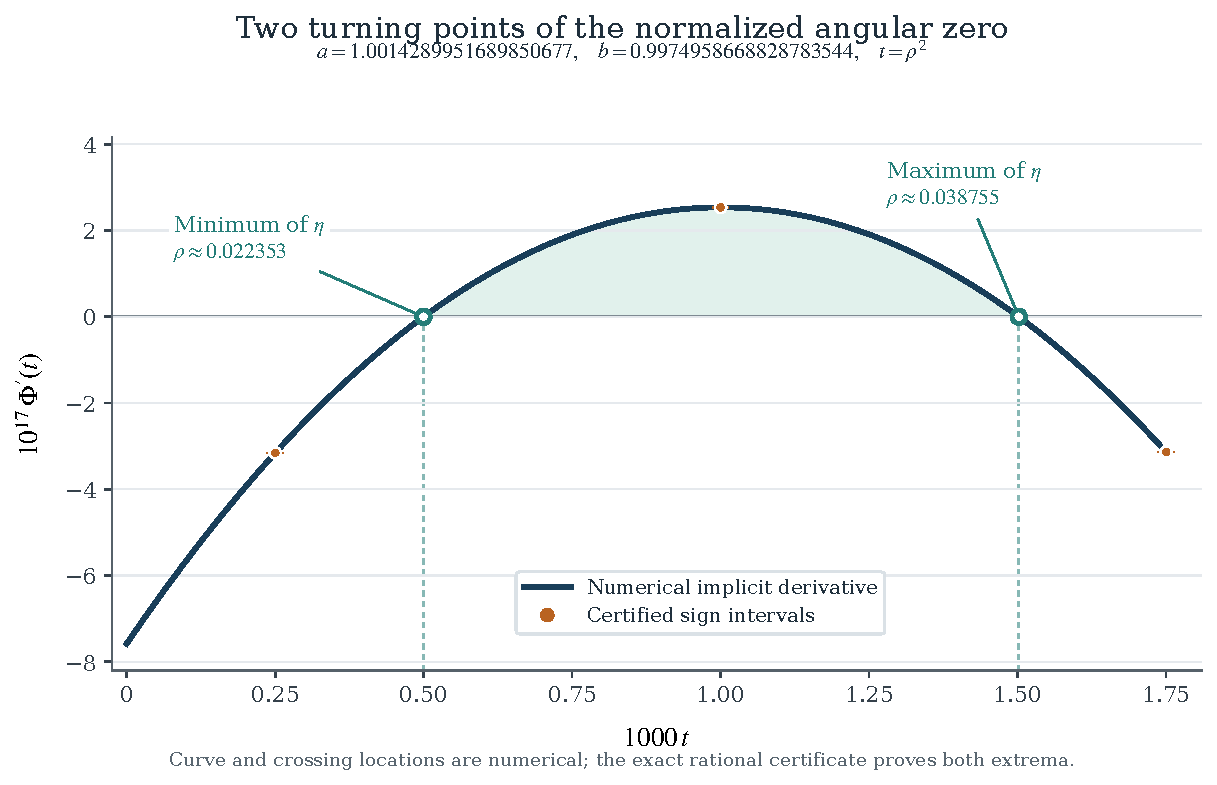
\includegraphics[width=\textwidth]{figures/radial_two_extrema.pdf}
\caption{The actual implicit derivative for the rational orders in
\eqref{rd:eq:explicitpair}. The blue curve and crossing locations
are numerical evaluations at 85 decimal digits; the orange markers
show the three exact rational sign enclosures. The independent
certificate proves $\Phi'''<0$ on the entire displayed interval,
so these signs establish exactly two simple critical points.
The much finer decimal crossing locations are diagnostic, not
additional certified radius brackets.}
\label{fig:radial-two}
\end{figure}

% Integration-ready research section. Parent supplies theorem environments,
% amsmath, amssymb, amsthm, and hyperref. Bibliography keys suggested below.
\section{A square-root transition in the late reflected residues}
\label{moderate:sec}

This section concerns a different simultaneous limit from the transition
$n/(m+1)-\log m=O(1)$ for the moments themselves. Here the late residue
index $k$ grows, and the reflected exponent is allowed to satisfy
$m=O(\sqrt{k})$. The fixed-$m$ asymptotic in the manuscript does not
cover this limit. The novelty assertion here is relative to the pinned
repository: no claim of priority over all literature is made. We prove a Gaussian damping factor, give its first
correction, and then obtain a sharp truncation theorem for a growing
reflected exponent.

Put
\[
 f(x)=\log\Gamma(x),\quad B(x)=\log\Gamma(1-x),\quad
 M_{n,m}=\int_0^1 f(x)^n f(1-x)^m\,dx,
\]
and retain the manuscript's residues
\begin{equation}\label{moderate:eq:A}
 A_{k,m}=\frac1k[x^{k-1}]\Gamma(1+x)^k B(x)^m.
\end{equation}
The parameters $k,m$ are integers with $k\ge1$, $m\ge0$.
The coefficients vanish when $k\le m$. In the meromorphic transform
$F_m(z)=\int_0^1\Gamma(x)^zB(x)^m\,dx$, the actual residue is
$\operatorname*{Res}_{z=k}F_m(z)=-kA_{k,m}$, so its sign is the
opposite of the coefficient sign. The standard Taylor series
for log gamma used below follows from DLMF, Section~5.7\cite{moderate:DLMF}.
Lagrange inversion and the underlying saddle and singularity methods are
classical\cite{moderate:Gessel,moderate:FS}; the moving-parameter estimates
are proved explicitly here.
Define
\[
 \phi(u)=\Gamma(1-u),\quad a(u)=-\log\Gamma(1+u),\quad D=u\frac d{du}.
\]
Let $\tau\in(0,1)$ be the unique solution of
$D\log\phi(\tau)=1$, and put
\begin{equation}\label{moderate:eq:constants}
 \rho=\frac{\tau}{\phi(\tau)},\quad
 \Lambda=-\log\rho,\quad b=a(\tau),\quad
 v=D^2\log\phi(\tau),\quad
 C=\frac{\tau}{\sqrt{2\pi v}}.
\end{equation}
All these constants are positive. Use a local real branch of $\log a$
at $\tau$ and set
\begin{equation}\label{moderate:eq:derivatives}
 r_j=D^j\log a(\tau),\qquad
 \kappa_j=D^j\log\phi(\tau),\qquad
 \delta_\Gamma=\frac{r_1^2}{2v}.
\end{equation}
Thus $\kappa_2=v$. The subscript on $\delta_\Gamma$ distinguishes this
constant from a small contour neighborhood.
The damping constant is strictly positive. Indeed
$D\log\phi(1/2)=\gamma/2+\log2<1$ and
$\psi(3/2)=2-\gamma-2\log2>0$, using
$\gamma<3/5$ and $\log2<7/10$. Hence $\tau>1/2$,
$\psi(1+\tau)>0$, and
$r_1=-\tau\psi(1+\tau)/b<0$.
Numerically,
\[
 b=0.1206254661326052\ldots,\quad
 r_1=-0.1684096130814827\ldots,\quad
 \delta_\Gamma=0.00624269203454726\ldots.
\]
These decimals only illustrate the constants; their defining equations
are used in the proof.

\begin{theorem}[Uniform late-residue transition]\label{moderate:thm:late}
Fix $L<\infty$. Uniformly for integers $0\le m\le L\sqrt{k}$ as
$k\to\infty$, with $\xi=m/\sqrt{k}$,
\begin{equation}\label{moderate:eq:late}
 A_{k,m}=(-1)^{k+m-1}C b^m\rho^{-k}k^{-3/2}
 e^{-\delta_\Gamma\xi^2}
 \left(1+\frac{P_1(\xi)}{\sqrt{k}}+O_L(k^{-1})\right),
\end{equation}
where
\begin{align}\label{moderate:eq:P1}
 P_1(\xi)={}&\left[-\frac{r_1+r_2/2}{v}
             +\frac{\kappa_3r_1}{2v^2}\right]\xi\notag\\
 &+\left[\frac{r_2r_1^2}{2v^2}
             -\frac{\kappa_3r_1^3}{6v^3}\right]\xi^3.
\end{align}
For every fixed $J\ge0$ there are explicitly computable real
polynomials $P_0,\ldots,P_J$, with $P_0=1$, such that the parenthesis
in \eqref{moderate:eq:late} equals
\[
 \sum_{j=0}^J k^{-j/2}P_j(\xi)
       +O_{L,J}(k^{-(J+1)/2}).
\]
In particular the coefficient signs are uniformly $(-1)^{k+m-1}$ for all
sufficiently large $k$ in this moving range. If $m/\sqrt{k}\to\xi_0$,
then the ratio of $A_{k,m}$ to its fixed-$m$ leading expression converges
to $e^{-\delta_\Gamma\xi_0^2}$.
\end{theorem}

\begin{proof}
Replacing $x$ by $-u$ in \eqref{moderate:eq:A} gives
\[
 A_{k,m}=\frac{(-1)^{k+m-1}}{k}
        [u^{k-1}]\phi(u)^k a(u)^m.
\]
The series of $\phi$ has strictly positive coefficients, because
\[
 \log\phi(u)=\gamma u+\sum_{j\ge2}\frac{\zeta(j)}j u^j.
\]
Consequently
\[
 Q(t)=\frac{\phi(\tau e^{it})}{\phi(\tau)}e^{-it}
\]
satisfies $|Q(t)|<1$ for $0<|t|\le\pi$, and
\[
 \log Q(t)=-vt^2/2-i\kappa_3t^3/6+\kappa_4t^4/24+O(t^5).
\]
Cauchy's coefficient formula is
\begin{equation}\label{moderate:eq:cauchy}
 A_{k,m}=\frac{(-1)^{k+m-1}\tau\rho^{-k}b^m}{2\pi k}
 \int_{-\pi}^{\pi}Q(t)^k e^{it}
       \left(\frac{a(\tau e^{it})}{b}\right)^m\,dt.
\end{equation}
No logarithm of $a$ on the full circle is required: $a^m$ is an analytic
integer power. Choose a small fixed $\epsilon>0$ such that $a$ is nonzero
near the arc $|t|\le\epsilon$. Outside that arc, compactness gives a
bound $O(q^k H^m)$ with $q<1$ and a fixed $H$. Since $m\le L\sqrt{k}$,
this is exponentially small in $k$.

On the small arc use the logarithm with value $\log b$ at zero.
Real Taylor coefficients imply
\[
 \log\frac{a(\tau e^{it})}{b}
 =ir_1t-r_2t^2/2-ir_3t^3/6+O(t^4).
\]
Its real part is $O(t^2)$. After reducing $\epsilon$ if necessary,
$|Q(t)|^k|a(\tau e^{it})/b|^m\le e^{-c kt^2}$ with $c>0$, uniformly
in the stated range once $k$ is large. Thus the portion
$k^{-2/5}\le|t|\le\epsilon$ is $O(e^{-c k^{1/5}})$.
Set $t=z/\sqrt{k}$ on the remaining arc. Its integrand is
\begin{align*}
 e^{-vz^2/2+ir_1\xi z}\bigg[1+\frac1{\sqrt{k}}
 \left(iz-\frac{i\kappa_3z^3}{6}-\frac{\xi r_2z^2}{2}\right)
 +O_L\left(k^{-1}(1+|z|^6)\right)\bigg].
\end{align*}
The error is bounded by an integrable polynomial times a fixed Gaussian;
this follows from the analytic Taylor remainder and the preceding
Gaussian bound. Extending the $z$ interval to $\mathbb R$ has an
exponentially small cost. The leading integral is
\[
 \int_{\mathbb R}e^{-vz^2/2+ir_1\xi z}\,dz
  =\sqrt{\frac{2\pi}{v}}e^{-r_1^2\xi^2/(2v)}.
\]
It is bounded away from zero relative to $\sqrt{2\pi/v}$ for
$0\le\xi\le L$, so all subsequent error estimates remain relative
and uniform.

Gaussian differentiation gives the normalized moments
\[
 \langle z\rangle=\frac{ir_1\xi}{v},\qquad
 \langle z^2\rangle=\frac1v-\frac{r_1^2\xi^2}{v^2},\qquad
 \langle z^3\rangle=i\left(\frac{3r_1\xi}{v^2}
                          -\frac{r_1^3\xi^3}{v^3}\right).
\]
Substituting these into the term of order $k^{-1/2}$ gives
\eqref{moderate:eq:P1}. For any higher fixed order, expand the two
analytic logarithms and $e^{it}$ to the corresponding finite order,
then integrate the resulting polynomial against this same complex
Gaussian. Gaussian domination bounds the remainder. Differentiation
of the Gaussian Fourier transform shows that every normalized
coefficient is a polynomial in $\xi$. This proves the full expansion
and all assertions of the theorem.
\end{proof}

A completely explicit coefficient prescription is available. With
$\varepsilon=k^{-1/2}$, expand
\begin{equation}\label{moderate:eq:algorithm}
 \exp\left\{i\varepsilon z+
 \sum_{j\ge3}\frac{\kappa_j(iz)^j}{j!}\varepsilon^{j-2}
 +\xi\sum_{j\ge2}\frac{r_j(iz)^j}{j!}\varepsilon^{j-1}\right\}
 =\sum_{j\ge0}T_j(z,\xi)\varepsilon^j.
\end{equation}
Then $P_j(\xi)$ is the integral of $T_j$ against
$e^{-vz^2/2+ir_1\xi z}$, divided by the leading Gaussian integral.
Only finitely many terms are needed for each $j$.
As a consistency check, the fixed-$m$ coefficient in the manuscript is
\[
 \beta_m=\beta_0+
 m\left[-\frac{r_1+r_2/2}{v}+\frac{\kappa_3r_1}{2v^2}\right]
 -\delta_\Gamma m^2.
\]
The quadratic term is exactly the first Taylor coefficient of the
Gaussian damping factor. The uniform theorem resums that part when
$m^2/k$ is no longer negligible.

\subsection{Uniform optimal truncation with a growing reflected exponent}

\begin{theorem}[A moving-exponent half-term law]\label{moderate:thm:half}
Fix $L,E<\infty$. Let $n,N\to\infty$ through positive integers,
$0\le m\le L\sqrt{N}$, and $|\eta|\le E$, where
$\eta=N\Lambda-n$. Then
\begin{align}\label{moderate:eq:half}
 \frac{M_{n,m}/n!-\sum_{k=1}^{N-1}A_{k,m}/k^n}{A_{N,m}/N^n}
 =\frac12+
 \frac{3/2-\delta_\Gamma m^2/N-\eta}{4N}
 +O_{L,E}(N^{-3/2}).
\end{align}
The denominator is nonzero for all sufficiently large $N$, uniformly
in the stated range. In particular the error is asymptotic to half the
first omitted term, and its eventual sign is $(-1)^{N+m-1}$.
The theorem supplies a proved growing range; it does not assert this
range is maximal.
\end{theorem}

\begin{proof}
We give the contour and tail details because neither a formal growing
substitution in the fixed-$m$ formula nor an infinite divergent Taylor
tail would justify this statement.
Let $h$ be the inverse germ $h=q\phi(h)$, let $g(t)=-h(-t)$, and set
\[
 W_m(x)=\int_0^x B(u)^m\,du,\qquad G_m(t)=W_m(g(t)).
\]
Lagrange inversion gives $G_m(t)=\sum_{k\ge1}A_{k,m}t^k$ near zero.
The manuscript's inverse-gamma argument shows that $g$ continues to a
slit disk of radius greater than $\rho$, whose only singularity on its
circle of convergence is at $-\rho$. For completeness, positivity of
the coefficients of $h$ gives $|h(q)|<\tau$ at every $|q|=\rho$,
$q\ne\rho$; then
$|q\phi'(h(q))|<\rho\phi'(\tau)=1$ allows analytic continuation.
At $q=\rho$ the first derivative of $u/\phi(u)$ vanishes and the second
does not, so ordinary local inversion gives a convergent square-root
expansion. Compactness produces a common slit disk. Shrink it so
$|g|<r_0<1$ there; this makes composition with every $W_m$ valid.

Choose a fixed outer radius $R>\rho$ in that disk and a small
$0<\epsilon<\Lambda$ with $\rho e^\epsilon<R$. Along its negative cut define
the real, possibly signed density
\[
 \nu_m(s)=\frac{(-1)^m}{2\pi i}
        \bigl(G_m(-s+i0)-G_m(-s-i0)\bigr),\qquad \rho<s<R.
\]
Put $\mathcal B_{N,m}=(-1)^{N+m-1}A_{N,m}$.
Cauchy contour deformation yields
\begin{equation}\label{moderate:eq:cut-coeff}
 \mathcal B_{N,m}=I_{N,m}+O(M^mR^{-N}),\qquad
 I_{N,m}=\int_\rho^R s^{-N-1}\nu_m(s)\,ds,
\end{equation}
for a fixed $M$, with an inessential enlargement of the constant.
The corresponding remainder contour has the additional kernel
$s/(s+t)$. The common factor and sign cancel after division by
$A_{N,m}t^N$. Outer-contour errors, including this division, are
exponentially small for $m\le L\sqrt{N}$ and
$\rho e^{-\epsilon}\le t\le\rho e^\epsilon$.

The jump need not be positive in this moving range. The needed absolute
bound is as follows. Write $u=(s-\rho)/\rho$. The square-root inverse
has $g(-s\pm i0)=-\tau+O(\sqrt{u})$ and a connecting path of length
$O(\sqrt{u})$. On that path
$|B(z)|\le b\exp(C_0\sqrt{u})$ for sufficiently small fixed $u$.
Since $W_m'=B^m$,
\[
 |\nu_m(\rho(1+u))|
 \le C_1 b^m\sqrt{u}\exp(C_0m\sqrt{u}).
\]
On the rest of the finite cut it is at most $C_2M^m$. Substituting
$w=Nu$, using $m\le L\sqrt{N}$ and
$(1+u)^{-N-1}\le e^{-cNu}$ on the small interval, proves for every
fixed $j\ge0$
\begin{equation}\label{moderate:eq:absolute-jump}
 \int_\rho^R \left|\frac{s-\rho}{\rho}\right|^j
    s^{-N-1}|\nu_m(s)|\,ds
 \le C_{L,j} b^m\rho^{-N}N^{-j-3/2}.
\end{equation}
The integrable majorant is a constant times
$w^{j+1/2}e^{-cw+C_0L\sqrt{w}}$.
By Theorem~\ref{moderate:thm:late}, division by $\mathcal B_{N,m}$
turns \eqref{moderate:eq:absolute-jump} into $O_{L,j}(N^{-j})$.
This absolute estimate prevents cancellation in the signed jump from
invalidating the Taylor-remainder bounds.

The first normalized cut moment is computed without expanding the
moving jump explicitly. The exact finite-cut identity gives
\[
 \int_\rho^R\frac{s-\rho}{\rho}s^{-N-1}\nu_m(s)\,ds
   =\rho^{-1}I_{N-1,m}-I_{N,m}.
\]
Use Theorem~\ref{moderate:thm:late} through order $N^{-1}$, with
relative remainder $O_L(N^{-3/2})$, both at $N-1$ and at $N$ with
the same $m$. The polynomials in that expansion are smooth for bounded
$m/\sqrt N$. Their ratio changes by $O_L(N^{-3/2})$, while the leading
factors give
\begin{align*}
 \frac{\mathcal B_{N-1,m}}{\rho\mathcal B_{N,m}}
 &=\left(\frac{N}{N-1}\right)^{3/2}
    \exp\left(-\frac{\delta_\Gamma m^2}{N(N-1)}\right)
    \bigl(1+O_L(N^{-3/2})\bigr)\\
 &=1+\frac{3/2-\delta_\Gamma m^2/N}{N}
       +O_L(N^{-3/2}).
\end{align*}
For $r=t/\rho$,
\[
 \frac{s}{s+t}=\frac1{1+r}+
            \frac{r}{(1+r)^2}u+O(u^2)
\]
uniformly on the fixed middle interval. Equations
\eqref{moderate:eq:cut-coeff}--\eqref{moderate:eq:absolute-jump} therefore give
\begin{align}\label{moderate:eq:inverse-remainder}
 \frac{G_m(t)-\sum_{k<N}A_{k,m}t^k}{A_{N,m}t^N}
 =\frac1{1+r}+
 \frac{r}{(1+r)^2}\frac{3/2-\delta_\Gamma m^2/N}{N}
 +O_L(N^{-3/2}).
\end{align}

It remains to justify averaging this local statement. The exact
layer-cake identity is
\[
 \frac{M_{n,m}}{n!}=\frac1{\Gamma(n)}
       \int_0^\infty y^{n-1}G_m(e^{-y})\,dy.
\]
After subtracting the finite sum, the ratio in
\eqref{moderate:eq:half} is the expectation of the left side of
\eqref{moderate:eq:inverse-remainder} at $t=e^{-Y}$, where $Y$ has
gamma shape $n$ and rate $N$.
Its probability outside $|Y-\Lambda|\le\epsilon$ is $O(e^{-cN})$
for bounded $\eta$, by the elementary gamma moment-generating function.
Uniform subexponential bounds on the normalized remainder suffice on
that complement. To obtain them, Cauchy's coefficient formula on
$|u|=\tau$ gives
\[
 |A_{k,m}|\le\frac{\tau}{k}\rho^{-k}H^m
\]
with a fixed $H$. Below $t=\rho e^{-\epsilon}$ sum the absolutely
convergent Taylor tail. Above $t=\rho e^\epsilon$ bound the finite
polynomial by its absolute terms. Division by the uniform lower bound
for $|A_{N,m}|$ in Theorem~\ref{moderate:thm:late} gives at most a
polynomial in $N$ times $e^{C_L\sqrt N}$ in both cases.
The remaining function term on the upper interval satisfies
$0\le G_m(t)\le m!$ for $0\le t\le1$: indeed $0\le g(t)\le1$
and $B(x)\le-\log(1-x)$, since
$\log\Gamma(2-x)\le0$ by log convexity between one and two. Thus
$W_m(g(t))\le\int_0^1[-\log(1-x)]^m\,dx=m!$.
After division its size is
at most a polynomial times
$e^{-\epsilon N}m!b^{-m}$, hence exponentially small in $N$ because
$m\log(m+1)=O_L(\sqrt N\log N)$.
The weighted outer contribution is therefore exponentially small.

Finally put $V=Y-\Lambda$. Then
\[
 \mathbb EV=-\eta/N,\quad \mathbb EV^2=O_E(N^{-1}),\quad
 \mathbb EV^3=O_E(N^{-2}),\quad \mathbb EV^4=O_E(N^{-2}).
\]
The leading kernel has expansion
$1/(1+e^{-V})=1/2+V/4-V^3/48+O(V^4)$, so its expectation is
$1/2-\eta/(4N)+O_E(N^{-2})$. The next kernel is
$e^{-V}/(1+e^{-V})^2=1/4+O(V^2)$, since its derivative vanishes
at zero. Its expectation is $1/4+O_E(N^{-1})$.
Averaging \eqref{moderate:eq:inverse-remainder} gives
\eqref{moderate:eq:half}. The signs and nonvanishing follow from
Theorem~\ref{moderate:thm:late}.
\end{proof}

\paragraph{What the theorem resolves and what it leaves open.}
The fixed-reflected-exponent warning in the manuscript is correct; it
should now be supplemented by a separate theorem for $m=O(\sqrt N)$.
The square-root scale is the first scale on which the leading late
residue changes by a nontrivial factor. It does not destroy the
half-term law, but it changes that law's first correction. The
fixed-$m$ correction $\beta_m/(4N^2)$ contains the same term
$-\delta_\Gamma m^2/(4N^2)$; the result above proves the relevant
resummation uniformly instead of substituting a growing parameter in
an uncontrolled remainder.

The next subsection proves a small proportional range for the
coefficients themselves. The maximal extent of that range and
extensions of the half-term remainder law are separate questions:
a coefficient asymptotic alone does not control a normalized
signed-cut remainder.

% Additional proved subsection, to follow moderate_reflection.tex.
% It uses that section's notation and does not enlarge the half-term theorem.
\subsection{A small proportional range and a second coefficient transition}
\label{moderate:sec:proportional}

The preceding circle argument also gives a nonzero proportional range
for the late coefficients themselves. This strengthens the Gaussian
formula without changing the stated range of the half-term remainder
law.

\begin{theorem}[Uniform small proportional saddle]
\label{moderate:thm:proportional}
There exists $c_0\in(0,1)$ with the following properties. For
$0\le c\le c_0$ there is a unique real-analytic continuation
$\tau_c$ of $\tau_0=\tau$ solving
\begin{equation}\label{moderate:eq:moving-saddle}
 D\log\phi(\tau_c)+cD\log a(\tau_c)=1.
\end{equation}
Its curvature
\[
 V(c)=D^2\log\phi(\tau_c)+cD^2\log a(\tau_c)
\]
is positive. Define
\begin{equation}\label{moderate:eq:rate-prefactor}
 S(c)=\log\phi(\tau_c)+c\log a(\tau_c)-\log\tau_c,
 \qquad C(c)=\frac{\tau_c}{\sqrt{2\pi V(c)}}.
\end{equation}
Uniformly for integers $0\le m\le c_0 k$, with $c=m/k$,
\begin{equation}\label{moderate:eq:proportional}
 A_{k,m}=(-1)^{k+m-1}C(c)k^{-3/2}e^{kS(c)}
                         \bigl(1+O(k^{-1})\bigr).
\end{equation}
There is a uniform expansion to every fixed order in integer powers of
$k^{-1}$, with real-analytic coefficient functions of $c$.
The constant $c_0$ is asserted to exist; no numerical lower bound for it
or maximality assertion is included.
\end{theorem}

\begin{proof}
Use the logarithmic radius $x=\log u$ and put
$f(x)=\log\phi(e^x)-x$, $g(x)=\log a(e^x)$ locally near
$x_0=\log\tau$. Then $f'(x_0)=0$ and $f''(x_0)=v>0$.
The analytic implicit-function theorem applied to
$f'(x)+cg'(x)=0$ supplies $x(c)=\log\tau_c$ near zero.
After shrinking the interval, $\tau_c$ lies in a fixed compact
$I\subset(0,1)$ where $a$ is positive, and $V(c)>v/2$.
Uniqueness here means uniqueness of this local continuation; it does
not classify other real or complex saddles.

Choose a small fixed angular neighborhood $|t|<\epsilon$ on which
$a(ue^{it})$ is nonzero for every $u\in I$. Positivity of the
Taylor coefficients of $\phi$ gives a strict uniform bound
\[
 q:=\sup_{u\in I,\ \epsilon\le|t|\le\pi}
         \frac{|\phi(ue^{it})|}{\phi(u)}<1.
\]
Also let
\[
 H=\max\left\{1,\sup_{u\in I,\ |t|\le\pi}
                   \frac{|a(ue^{it})|}{a(u)}\right\}<\infty.
\]
Further decrease $c_0$ so that $qH^{c_0}<1$. In the Cauchy integral
on $|u|=\tau_c$, the outer arc divided by the positive saddle
amplitude is at most $q^kH^m\le(qH^{c_0})^k$.
This is the global estimate needed for proportional $m$: no logarithm
or fractional power of $a$ on the full circle is assumed.

On the small arc the normalized local logarithmic phase is
\[
 f(x(c)+it)-f(x(c))
     +c\bigl(g(x(c)+it)-g(x(c))\bigr).
\]
Its linear term vanishes by \eqref{moderate:eq:moving-saddle}; its
quadratic term is $-V(c)t^2/2$. Analyticity, reality on the real
radius, and compactness give a uniform Gaussian modulus bound for
a sufficiently small fixed $\epsilon$. Choose this $\epsilon$ first
and then make the preceding final reduction of $c_0$, so the outer-arc
estimate uses the same angular neighborhood. Taylor expansion with $t=z/\sqrt k$ and
amplitude $e^{it}$ now gives
\[
 \int e^{k\{f(x(c)+it)-f(x(c))
                +c[g(x(c)+it)-g(x(c))]\}}e^{it}\,dt
 =\sqrt{\frac{2\pi}{kV(c)}}\bigl(1+O(k^{-1})\bigr).
\]
The discarded arcs are exponentially small. Odd terms integrate to
zero, so only integer powers of $k^{-1}$ occur. Analyticity and
uniform derivative bounds also prove the asserted all-orders
expansion. Restoring the Cauchy prefactor
$(-1)^{k+m-1}\tau_c e^{kS(c)}/(2\pi k)$ proves the theorem.
\end{proof}

\begin{corollary}[Explicit rate expansion and cubic transition]
\label{moderate:cor:cubic-transition}
Put
\begin{align*}
 d_1&=-\frac{r_1+r_2/2}{v}+\frac{\kappa_3r_1}{2v^2},\\
 d_3&=\frac{r_2r_1^2}{2v^2}-\frac{\kappa_3r_1^3}{6v^3}.
\end{align*}
Then
\begin{align}\label{moderate:eq:analytic-rate}
 S(c)&=\Lambda+c\log b-\delta_\Gamma c^2+d_3c^3+O(c^4),\notag\\
 C(c)&=C\bigl(1+d_1c+O(c^2)\bigr).
\end{align}
Consequently the Gaussian-resummed leading expression
\begin{equation}\label{moderate:eq:extended-Gaussian}
 A_{k,m}\sim(-1)^{k+m-1}Cb^m\rho^{-k}k^{-3/2}
                     e^{-\delta_\Gamma m^2/k}
\end{equation}
is uniform for $m=o(k^{2/3})$: precisely, it holds uniformly for
$0\le m\le\varepsilon_k k^{2/3}$ whenever $\varepsilon_k\to0$.
For each fixed $L<\infty$, uniformly for $0\le m\le Lk^{2/3}$,
\begin{equation}\label{moderate:eq:cubic-uniform}
 A_{k,m}=(-1)^{k+m-1}Cb^m\rho^{-k}k^{-3/2}
  \exp\left(-\frac{\delta_\Gamma m^2}{k}
               +\frac{d_3m^3}{k^2}\right)
           \bigl(1+O_L(k^{-1/3})\bigr).
\end{equation}
In particular, if $m/k^{2/3}\to\chi\ge0$, the ratio to the right-hand
leading expression in \eqref{moderate:eq:extended-Gaussian} tends to
$e^{d_3\chi^3}$. The numerical value is
$d_3=-0.00545592970200504\ldots$; the exact defining formula is used
in the theorem.
\end{corollary}

\begin{proof}
Differentiating the saddle equation at zero gives
$x'(0)=-r_1/v$. Since $S(c)=f(x(c))+cg(x(c))$ and
$f'(x(c))+cg'(x(c))=0$, expansion through degree three gives
\[
 S(c)=\Lambda+c\log b-\frac{r_1^2}{2v}c^2+
       \left(\frac{r_2r_1^2}{2v^2}
             -\frac{\kappa_3r_1^3}{6v^3}\right)c^3+O(c^4).
\]
For the prefactor,
\[
 (\log C)'(0)=x'(0)-\frac{\kappa_3x'(0)+r_2}{2v}=d_1.
\]
This proves \eqref{moderate:eq:analytic-rate}. Upon setting $c=m/k$,
Theorem~\ref{moderate:thm:proportional} becomes
\begin{align*}
 A_{k,m}={}&(-1)^{k+m-1}Cb^m\rho^{-k}k^{-3/2}
 e^{-\delta_\Gamma m^2/k}\,
 \exp\left(\frac{d_3m^3}{k^2}+O\left(\frac{m^4}{k^3}\right)\right)\\
 &\hspace{4em}\times\left(1+\frac{d_1m}{k}
                  +O\left(\frac{m^2}{k^2}+\frac1k\right)\right).
\end{align*}
For $m=o(k^{2/3})$ all corrections on the last two factors tend to
one uniformly. For $m\le Lk^{2/3}$, the quartic rate error and the
first prefactor correction are $O_L(k^{-1/3})$, which gives
\eqref{moderate:eq:cubic-uniform} and its limiting assertion.
Finally, when $m=\xi\sqrt k$, the prefactor and cubic rate contribute
$(d_1\xi+d_3\xi^3)/\sqrt k$. This is exactly $P_1(\xi)$ in
\eqref{moderate:eq:P1}, independently matching the square-root
calculation.
\end{proof}

\begin{proposition}[Strict cubic damping]
\label{moderate:prop:cubic-negative}
The exact cubic rate coefficient satisfies $d_3<0$.
Thus the transition factor $e^{d_3\chi^3}$ is strictly below one
for every $\chi>0$.
\end{proposition}
\begin{proof}
We already know $\tau>1/2$ and $r_1<0$. The positive log-gamma
series also gives
\[
 D\log\phi(3/5)>
 \frac12\frac35+\frac{(3/5)^2}{1-3/5}
 =\frac65>1,
\]
so $\tau<3/5$. Put $P=\psi(1+\tau)$ and
$Q=\psi'(1+\tau)$. The trigamma series and its
derivatives~\cite{moderate:DLMF} show that $\psi$ is increasing
and concave and that
\[
 Q=\sum_{n\ge0}\frac1{(1+\tau+n)^2}>
       \frac1{1+\tau}.
\]
Using $\gamma>1/2$, $\log2>2/3$, and $\pi^2<10$ in the
classical values at $3/2$ gives
\[
 0<P<\psi(3/2)+\frac1{10}\psi'(3/2)
       <\frac16+\frac1{10}=\frac4{15},
 \qquad
 \tau Q>\frac{\tau}{1+\tau}>\frac13.
\]
In particular $P<\tau Q$.

Write $T=\psi'(1-\tau)>0$. Termwise comparison in the
polygamma series yields
$-\psi''(1-\tau)\le2T/(1-\tau)$. At the saddle,
\[
 v=1+\tau^2T,\qquad
 \kappa_3=1+3\tau^2T-\tau^3\psi''(1-\tau).
\]
Since $\tau<3/5$, these imply
$\kappa_3<1+6\tau^2T<6v$, or $\kappa_3/(3v)<2$.
Finally,
\[
 r_1=-\frac{\tau P}{b},\qquad
 r_2=r_1-r_1^2-\frac{\tau^2Q}{b}.
\]
Because $r_1<0$,
\[
 r_2-\frac{\kappa_3r_1}{3v}
 <-r_1-r_1^2-\frac{\tau^2Q}{b}
 =\frac{\tau}{b}(P-\tau Q)-r_1^2<0.
\]
Multiplication by $r_1^2/(2v^2)>0$ proves the assertion.
\end{proof}

The proportional theorem settles existence of a small positive sector.
The remaining question is its maximal extent: determine when another
arc or saddle becomes competitive and how that affects coefficient
signs. The cut-density estimates in the half-term theorem normalize by
an exponentially damped coefficient and were proved only for bounded
$m/\sqrt N$; the new coefficient theorem alone does not enlarge that
remainder theorem.

\section{Audit, corrections, and verification}
\label{sec:audit}

The source audit was performed against the exact commit specified on
the title page. It was selective and mathematical: we checked the
definitions and proof dependencies needed for the four continuations,
then compared the conclusions with the manuscript's explicit open
questions. This is not an assertion that every formula in the entire
repository has been independently re-proved.

\subsection{A wording correction concerning non-elementarity}

The paragraph preceding Equation~\texttt{vertical:eq:Im3} in
\src{chapters/03-algebraic.tex} describes the imaginary part of
$\Li_3(1+i)$ as \emph{no longer elementary at all}. The displayed
hypergeometric representation does not establish that assertion.
An exact expression in terms of a central-binomial tower constant
is an evaluation in a specified language. It is not a proof that
the value cannot belong to some smaller algebra of constants.
Indeed, without specifying the meaning of elementary for a
number, the assertion has no definite mathematical test.

\begin{samepage}
A precise replacement is:
\begin{quote}
The imaginary part at $1+i$ is represented here by the
central-binomial Gaussian tower constant:
\end{quote}
\end{samepage}
followed by the existing, unchanged equation, and then:
\begin{quote}
This representation does not establish non-reducibility to a
specified smaller algebra of constants.
\end{quote}
The preceding claim that the general real part \emph{does not close}
should similarly be scoped to the computation being described.
One can say that differentiating and integrating the displayed
formula introduces an inverse-tangent-square integral, and that
no general reduction of that integral is supplied there.
This is a correction to the strength of the prose; the displayed
special-value formulas are not contradicted by this audit.
An exact-context patch implementing these two edits is included
in \src{integration/non_elementarity_wording.patch}.

\subsection{Statements that should be updated after integration}

\paragraph{Uniform Euler error.}
The warning that a bound on $|g_{a,b}|$ is insufficient to control
$2^N(E_N-g_{a,b})$ was correct. The explicit calculation in
Section~\ref{sec:euler} shows $R_2(1,1)>R_1(1,1)$.
Theorem~\ref{thm:Euler-uniform} now supplies the missing uniform
comparison. The open-status sentences in the subcritical and
real-order Euler sections should therefore be replaced by a
reference to the new theorem. The sharper constant $1$ on the
restricted domain $a\geq1$ remains useful and should be retained.
A global budget of $57/50$ is convenient, but it is not the sharp
bound on every subdomain.

\paragraph{Quartic threshold.}
The final paragraph of \src{chapters/05-real-turning.tex} correctly
labels its approximate simultaneous zero as diagnostic. Our exact
rectangle and derivative certificate promote that particular
location, its local uniqueness, and its sixth-order behavior to
theorems. They do not establish uniqueness on all $0<b<1$.
The current existence proof based on opposite signs of the quartic
coefficient remains a useful conceptual introduction. It should
be followed by the new local classification and explicit rational
two-extremum example, with a separate global open question.

\paragraph{Reflected coefficients and residues.}
The coefficient $A_{k,m}$ defined by Lagrange inversion and the
meromorphic residue are related by
\[
 \operatorname*{Res}_{z=k}
 \int_0^1\Gamma(x)^z\log^m\Gamma(1-x)\,dx=-kA_{k,m}.
\]
Any compact description of signs should retain this factor.
The moving-parameter theorems extend the fixed-$m$ estimates;
they do not justify inserting an arbitrary growing $m$ into a
fixed-parameter error term. The moment transition governed by
$n/(m+1)-\log m$ is a different simultaneous limit and should
remain separately indexed.

\paragraph{Height-one reductions and the literature.}
The Nielsen-polylogarithm work of Charlton, Gangl, and Radchenko
is a necessary part of the attribution for
Section~\ref{gorbit:sec:main}. In particular, the weight-seven
height-one reduction is an established functional equation.
Our presentation supplies a directly replayable shuffle
certificate, an explicit product correction, and a comparison
with the full binary quotient. The finite-direction formula
is stated in that full quotient, with its precise relation
space visible. Even when a formal obstruction is nonzero,
it must not be described as a proof that a complex number
cannot reduce.

\paragraph{Unresolved evaluations.}
The $S_6$ and revised $S_8$ candidates in the existing discovery
ledger remain conjectural. Neither the new Euler budget, a very
small residual, nor a formal obstruction to one reduction method
proves or disproves these special-value identities. This article
does not alter their evaluation status.

\subsection{The finite arithmetic proofs}

The exact programs use Python integers and
\src{fractions.Fraction}. No binary floating-point comparison
decides the sign of an interval in these proofs. The use of
Python is an implementation choice, not a trust claim about
all software: the written formulas specify finite statements
that can be replayed in another exact-arithmetic environment.
These are computer-assisted arithmetic proofs, not
proof-assistant formalizations.

\begin{longtable}{@{}>{\raggedright\arraybackslash}p{0.26\textwidth}>{\raggedright\arraybackslash}p{0.40\textwidth}>{\raggedright\arraybackslash}p{0.27\textwidth}@{}}
\toprule
Verifier & Exact task & Logical role\\
\midrule
\endhead
\src{verify_euler.py}
& Thirty-one rational axis enclosures, the rational global
budget, selected rational-order enclosures, and corrupted
candidate controls.
& Proves the finite inequalities used in
Proposition~\ref{prop:rational-budget}.\\[5pt]
\src{verify_depth_orbits.py}
& Exact Lyndon-bracket pairings, word-rank calculations,
the weight-seven product expansion, and the weight-eight
annihilator.
& Finite proof certificates for the explicit identities;
finite corroboration of the all-weight rank theorem.\\[5pt]
\src{certify_radial_degeneracy.py}
& Outward intervals for the simultaneous-zero rectangle,
the endpoint signs, the Jacobian, and the sixth coefficient.
& Supplies the finite sign claims needed for the analytic
existence and unfolding proof.\\[5pt]
\src{certify_two_extrema.py}
& Traps the actual implicit zero; bounds the infinite
series and its mixed derivatives; proves three signs
and uniform strict concavity.
& Proves the two-extremum statement for the exact
rational parameter pair.\\
\bottomrule
\end{longtable}
\addtocounter{table}{-1}

The Euler verifier also checks $6120$ rational kernel instances.
That grid is a useful regression check; the all-$N$ kernel theorem
is proved by the probability-mixture argument, not by extrapolation
from the grid. Its two deliberately false controls are a proposed
global constant $1$ and the changed finite value
$E_2(1,1)=-1/7$. The first is rejected by a certified analytic
enclosure; the second is rejected by exact rational evaluation,
which gives $-1/8$.

The word-rank checks through weight ten cover $25$ weight-depth
cases for each of the six-map and full-linear spans, and $34$
additional finite-direction cases. They are deliberately computed
from the expanded free-Lie words rather than by reusing the
dimension formula as the answer. The height-one membership checks
also test the asserted threshold on individual words. The
weight-eight obstruction is checked on $222$ transformed seed
words and $1792$ shuffle products. The weight-seven product
correction contains $864$ collected monomials; expanding their
shuffle products reproduces the residual word combination
exactly.

The first radial certificate uses a $2^{-192}$ outward grid.
Its logarithms are bounded by an atanh series with an explicit
geometric remainder, and exponentials by a positive Taylor sum
and a geometric tail. The second certificate range-reduces
logarithms before applying the same principle. The programs
record both the raw rational intervals and the simpler rational
enclosures printed in the theorems. Very small positive or
negative quantities are therefore proved to have their asserted
signs; their size is not inferred from decimal precision alone.

\subsection{Numerical diagnostics and independent review}

The optional numerical programs require \src{mpmath}, and the
asymptotic symbolic checks additionally use \src{sympy}.
They serve a different purpose from the exact programs.
The complete weight-seven functional identity, including
endpoint constants and products, was checked by direct disk
series at $z=1/4$ and $z=1/3$ with $80$ working decimal digits.
The discrepancies were approximately $3.7\cdot10^{-80}$ and
$2.1\cdot10^{-80}$. The proof comes from the exact word
identity and the branch argument; these numerical values
check their implementation.

The proposed sharp rate for $C_N-1$ is accompanied by $210$-digit
axis calculations and a few positive-$a$ checks. The latter replace
$g_{a,b}$ by $E_{512}$, with analytic contribution to the scaled
truncation error at most $(5/4)2^{N-512}$. That proved truncation
bound is separate from floating-point error. Neither these values
nor the numerical axis stationary points certify a global maximum.

For the reflected coefficients, the diagnostic data use $180$
working digits, compare two cases with independent Cauchy
quadrature, and repeat the six direct scaled-moment integrals
at $215$ digits. The repeated moment ratios differed by less
than $1.5\cdot10^{-108}$ in those cases. These are high-precision
agreements, not rigorous interval error bounds.
The accompanying tables retain examples outside the visible
asymptotic regime, including large normalized deviations at
moderate indices. Suppressing those rows would obscure the
meaning of a uniform theorem whose constants depend on a
fixed range parameter.

\begin{table}[tbp]
\centering
\small
\begin{tabular}{@{}rrrll@{}}
\toprule
$N$ & $n$ & $m$ & Observed normalized remainder
& First-correction prediction\\
\midrule
24 & 30 & 5  & $0.5127180890556$ & $0.5116978569285$\\
24 & 30 & 15 & $2.1726463253744$ & $0.5111559565783$\\
48 & 61 & 7  & $0.5094463157920$ & $0.5091282364092$\\
48 & 61 & 21 & $0.6787471547306$ & $0.5088627052376$\\
96 & 121 & 10 & $0.5027543017622$ & $0.5026340767530$\\
96 & 121 & 29 & $0.5028409944568$ & $0.5025085929532$\\
\bottomrule
\end{tabular}
\caption{Diagnostic values for the left side of
\eqref{moderate:eq:half}, compared with
$1/2+(3/2-\delta_\Gamma m^2/N-\eta)/(4N)$.
All six rows are retained, including the substantial
preasymptotic deviations at larger $m$ and smaller $N$.
The observed values are high-precision quadrature
results, not interval enclosures.}
\label{tab:half-diagnostics}
\end{table}

The four main arguments received separate mathematical
cross-checks during preparation. In particular, the endpoint
corrections in the Nielsen identity, the coefficient-dual
normalization in the binary-form calculation, the signed-cut
normalization in the half-term theorem, and the complete
implicit-derivative certificate for the explicit radial example
were checked independently of their initial derivations.
This record describes the scope of review; it is not a
substitute for external peer review.

\subsection{Reproduction and integration}

The archive includes a single entry point,
\src{code/reproduce.py}, which runs the exact verifiers without
requiring access to the original repository. Optional switches
replay the numerical diagnostics and regenerate the figures.
The figures are explanatory numerical plots; their captions
identify the exact statements that supply proof.
Run \src{latexmk -pdf article.tex} from the package root to
rebuild the document using the supplied section and figure files.

The provenance directory records the pinned commit, the
relative source paths used in the audit, and their SHA-256
digests. The integration guide maps each section and certificate
to the appropriate manuscript chapter. It also records the
small preamble requirements and label prefixes, so that the
standalone article can be integrated without depending on an
unstated local macro package. No changes were applied to the
source repository.

\section{Further research: precise questions and next steps}
\label{sec:research}

The results above close several concrete gaps, but each also
identifies a natural boundary. The following programme separates
conjectures with specific existing evidence from broader questions.
The proposed tasks are intended to lead to additional theorems
or falsifiable identities, not merely more decimal tables.

\subsection{Euler bounds: rates, extremizers, and further moment families}

\paragraph{Sharp bounds for a fixed truncation index.}
The global constant $C_*$ is forced by $N=1$ and $a\downarrow0$.
For practical computations with large $N$, it leaves substantial
room. Define the exact pointwise envelope
\[
 K_N(v)=\max_{0\leq x\leq1}\{W_N(vx)-W_N(x)\},
 \qquad 0<v<1.
\]
Theorem~\ref{thm:kernel} determines the supremum over all $N$,
but does not determine $K_N(v)$ in a useful closed form for
$N\geq2$. Find its maximizing point, its dependence on $N$,
and the strongest integrated bound it yields for fixed $a,b$.
A derivative equation for the maximizing point is elementary,
so the challenge is an interpretable exact inequality rather
than a numerical maximization.

The scaling $x=y/N$ suggests the limiting comparison
$e^{-vy}-e^{-y}$, whose maximum is
$(1-v)v^{v/(1-v)}$. This suggests asking for an error-controlled
limit of $K_N(v)$, including its behavior as $v\downarrow0$
and $v\uparrow1$. Uniformity at those endpoints matters
before integrating against an order-dependent measure.
The elementary limiting calculation alone does not supply
that uniformity.

\paragraph{Fractional-order late Euler errors.}
The integer-order manuscript already gives a polynomial in
$\tfrac12\log N$ multiplying $2^{-N}N^{-1/2}$, with leading
coefficient determined by the total weight. Extend the full
expansion to positive nonintegral $a,b$, explicitly tracking
the extra endpoint terms that appear when an exponent crosses
an integer. In particular, establish a uniform version of the
fixed-order leading behavior suggested by the two-measure
convolution,
\[
 E_N-g_{a,b}\sim
 \frac{\sqrt{\pi}}{2^{a+b}\Gamma(a+b)}
 \frac{2^{-N}(\log N)^{a+b-1}}{\sqrt N}.
\]
For positive integral orders this is already a theorem in
\src{chapters/05-signed-kernels.tex}; the research target is
the fractional continuation and its uniform error structure.
A proof should separate the region where both logarithmic
moment variables are large from the boundary layers in which
only one is large. The signed-measure representation can fail
to have finite mass, so the positive two-measure difference
is a promising starting point.

\paragraph{The rate of approach to the asymptotic global constant.}
Theorem~\ref{thm:euler-asymptotic-budget} proves $C_N\to1$, and
Proposition~\ref{prop:euler-axis-lower} gives a concrete lower
asymptotic. The natural next target is the matching upper bound.

\begin{conjecture}[Asymptotic optimal Euler constant]
\label{conj:euler-rate}
With
\[
 p=\frac{\log2}{\log(3/2)},\qquad
 q=\frac{\log3}{\log2},\qquad c=(1-q^{-1})q^{-p},
\]
the optimal scaled-error constant satisfies
\[
 C_N-1\sim cN^{-p}.
\]
\end{conjecture}

The matching lower bound is proved. The global upper bound over
positive $a$ is open, and even the sharp upper asymptotic for
the supremum over all $b$ on the axis requires an argument.
The moving-order phase law supplies a broad region with $R_N\to1$,
but that limit does not distinguish errors of order $N^{-p}$.
Any statement about near maximizers must specify the accuracy:
an error $o(C_N-1)$ is relevant here, whereas an error merely
$o(1)$ need not force $a\to0$. Monotonicity of $C_N$ is also
not asserted.

The diagnostic program \src{code/axis_remainder_diagnostics.py}
evaluates finite Euler sums at $210$ decimal digits.
For the following indices it finds numerical axis stationary
points, with the displayed scaled excess:
\begin{center}
\small
\begin{tabular}{@{}rrrr@{}}
\toprule
$N$ & $\widehat b_N$ & Stationary $b$ &
$(R_N(0,b)-1)/(cN^{-p})$\\
\midrule
4   & 4.5549051506  & 4.7024351462  & 0.8809410\\
16  & 7.9739277333  & 7.8500957399  & 1.0384240\\
64  & 11.3929503160 & 11.2260085539 & 1.0760668\\
256 & 14.8119728987 & 14.6711951089 & 1.0684372\\
\bottomrule
\end{tabular}
\end{center}
Their global optimality is not certified. At $b=\widehat b_N$,
the three tested positive values $a=10^{-4},10^{-2},10^{-1}$
all give smaller remainders than $a=0$. These are limited axis
and local checks; they do not establish the conjecture or
monotone convergence of the displayed ratios. An effective
compact-rectangle estimate, combined with a sharp analysis
of the axis scaling, is one possible route to an upper bound.

\paragraph{Further moving-order boundaries.}
Theorem~\ref{thm:euler-moving} treats two orders growing
proportionally to $\log N$. Determine the finer behavior
when one of the leading coefficients $A,B$ tends to zero,
or when one order remains fixed while the other crosses
the logarithmic threshold. The bounded-width gamma variable
then interacts with the smoothed threshold itself, and the
two normal profiles need not describe the first correction.
Also study orders tending to zero, where endpoint
concentration affects the fractional late-error expansion.
A useful result would connect the several scaling regimes
with explicit overlapping error bounds.

\paragraph{Other moment products.}
Theorem~\ref{thm:moment-general} applies to any two finite
positive measures. Explore shifted harmonic numbers,
Hurwitz-type inner sums, mixtures of orders, and products
arising from completely monotone sequences. For each family,
identify the sharp measure-specific constant rather than
automatically using $(1+\sqrt2)/2$.
Higher-depth nested partial sums lead to higher divided
differences of the same kernel. Determine which of those
differences have a fixed sign and what sharp moduli replace
the two-point inequality. This is a concrete route toward
certified Euler algorithms for real-order higher-depth
polylogarithms.

\subsection{Formal depth and genuine functional reduction}

\paragraph{Exploit the full binary formula constructively.}
The finite-direction dimension theorem gives the rank but
does not choose the best basis for an identity search.
Construct rational bases adapted to the irreducible
$\operatorname{Sym}^{w-2j}V\otimes\det^j$ summands and
their confluent interpolation conditions. This should make
it possible to solve reduction problems without forming
all $2^w$ words. The weight-seven product correction is
explicit but lengthy; a basis respecting reversal,
complementation, and endpoint regularization may produce a
much shorter analytic expression.

\paragraph{Compare with the Nielsen literature at each weight.}
The height-one results must be compared with the known
Nielsen reductions, including their meaning modulo products
and their exact symbol spaces. A useful next deliverable is
a table that gives, for every weight in a practical range,
the published reduction, a word certificate in the repository's
conventions, and the endpoint correction on a stated branch
domain. It should identify equivalence of relations, not
count the same identity multiple times because of a change
of notation.

\paragraph{Go beyond three punctures.}
The six transformations act on only three projective letter
directions. A general rational substitution may introduce
additional singularities and therefore a larger alphabet;
it is not represented by an arbitrary $2\times2$ change of
the old letters. Extend the rank problem to a specified
puncture set and a specified collection of rational maps.
Describe the kernel of specialization back to the original
periods. The weight-eight obstruction here is a useful test
case: which genuinely new pullbacks or distribution
relations remove it, and what new constants do they introduce?

\paragraph{Separate formal and period questions.}
For the unresolved Gaussian $S_6$ and $S_8$ evaluations,
specify the expected algebra of constants before searching.
Construct the corresponding functional relation space,
map it to the target specialization, and compare the proposed
identity with that image. A formal failure would indicate
that the chosen tools are insufficient. It would not prove
period independence. Conversely, an exact functional
certificate with controlled endpoint constants would settle
an evaluation without relying on an integer-relation residual.

\subsection{The global radial phase portrait}

Let $a_*(b)$ be the already proved unique solution of $K=0$
in $(1,2)$ for $0<b<1$, and put $q(b)=Q(a_*(b),b)$.
The pinned manuscript proves opposite signs at two rational
parameters and reports a wider diagnostic scan. The exact
certificate here proves one simple zero near the upper
endpoint of that interval.

\begin{conjecture}[Unique quartic transition on the quadratic threshold]
\label{conj:quartic-global}
The function $q$ has exactly one zero on $0<b<1$, namely
the certified $b_\dagger$. It is negative for
$0<b<b_\dagger$ and positive for $b_\dagger<b<1$.
\end{conjecture}

The local sign at the certified zero is proved, and the
existing finite scan supports the global statement. Neither
fact excludes additional zeros away from the isolating box.
A rigorous approach should combine asymptotic analysis as
$b\downarrow0$ and $b\uparrow1$ with a finite interval cover
of the remaining compact region. Direct interval evaluation
may be inefficient near $b=1$, where several low-order
coefficients nearly cancel. Factoring the known degeneration
at $(a,b)=(1,1)$ before bounding remainders is likely to be
essential.

\paragraph{Global continuation of the two-extremum region.}
The local fold and the explicit rational example prove that
a minimum followed by a maximum can occur. Follow the two
critical branches to larger radii and determine how they
end: collision, escape through $\rho=1$, or interaction with
another branch. Can more than two radial critical points
occur for some positive orders? The local concavity proof
does not address this global question. A plausible first
step is an interval continuation of the coupled equations
for the angular zero and its radial derivative, with a
separate proof that no branch is missed.

\paragraph{The older integer-order monotonicity question.}
The conjectured full-radius decrease for integer $a\geq2$,
and the special $a=1$ behavior, remain interesting.
The fractional examples do not refute them: their parameters
are close to, but different from, $(1,1)$.
Look for a sign-definite integral expression for the radial
derivative in the integer range. A proof based only on the
coefficient $K$ would establish local behavior and leave the
rest of the radius interval untreated.

\paragraph{Higher degeneracies.}
The binomial implicit equation gives every radial coefficient
without guessing higher Chebyshev expansions. Search for
families with $K=Q=R=0$ after adding a deformation parameter,
such as a Lerch shift or an extra inner moment. If a first
nonzero coefficient appears at $\rho^{2\ell}$, generic
one-parameter perturbation suggests turning radii with
power $1/(2\ell-2)$. State the transversality hypotheses
explicitly and prove the local normal form before drawing
a global bifurcation diagram.

\subsection{Growing reflected exponents and optimal truncation}

\paragraph{The maximal proportional-exponent regime.}
The shifted-saddle continuation establishes a nonzero
interval of proportional growth. Determine the largest
admissible interval by analyzing the real saddle equation
and competing complex saddles. Positivity of the Taylor
coefficients of $\Gamma(1-u)$ is available, but
$-\log\Gamma(1+u)$ does not have a positive coefficient
sequence. A local stationary point alone therefore does
not prove global contour dominance for all $m/k$.
Locate the first loss of dominance or the first saddle
collision, and give an exact or certified description of
the transition.

\paragraph{Move the optimal truncation index as well.}
When $m/N$ is no longer small, the exponential rate of the
coefficients changes. The optimal truncation index must
then be determined from that joint rate, rather than
retaining $N\Lambda\approx n$ without adjustment.
Derive the correct stationarity equation when $n,m,N$
grow together, and test whether a half-term law persists.
The signed jump on the negative cut requires absolute
moment estimates; eventual coefficient signs do not by
themselves make the cut density positive.

\paragraph{Effective constants and preasymptotic behavior.}
Turn the present uniform big-$O$ statements into explicit
inequalities in a chosen practical range. The diagnostic
examples show why this matters: a fixed range parameter
can be mathematically admissible while its asymptotic
behavior appears only at much larger indices.
Effective contour radii, bounds on logarithmic derivatives,
and a computable separation of the central arc from the
outer contour would turn the theorem into a usable
certified truncation prescription.

\paragraph{Connect the different moment scales.}
The coefficient scale $m\asymp\sqrt{k}$ and the direct-moment
scale involving $n/(m+1)-\log m$ arise from different
representations. Determine their overlap after the
optimal index is chosen, and compare the resulting
asymptotic expansions term by term. A matching theorem
would explain which representation is stable in each
region and where cancellations make one numerically
preferable.

\subsection{A practical order of attack}

The most bounded next tasks are an exact global sign study
for $q(b)$, a basis-efficient implementation of the finite-direction
rank theorem, and effective constants for the shifted saddle.
Each has a clearly specified output and can be checked
against the certificates in this article. The longer
projects are a global radial classification, an extension
to larger puncture alphabets, and a joint optimal-truncation
theory for proportional reflected exponents. The special-value
conjectures should remain visible throughout, but their
status should change only when an exact functional or
arithmetic certificate becomes available.

{\small\begin{thebibliography}{99}
\bibitem{ProveItSnapshot}
Vladimir Reshetnikov, \emph{ProveIt: Analysis / Polylogarithms},
consolidated manuscript and companion reports,
repository snapshot \src{3447bc59b78d138a7f0d536b66ac6e5cc5d5e49f},
consulted 10 October 2026.
\url{https://github.com/VladimirReshetnikov/ProveIt/tree/3447bc59b78d138a7f0d536b66ac6e5cc5d5e49f/Analysis/Polylogarithms/docs/manuscript}.
The source paths and their hashes used in this continuation are listed
in \src{provenance/baseline.json}.

\bibitem{DLMFEuler}
NIST Digital Library of Mathematical Functions,
Section 3.9, \emph{Acceleration of Convergence}, especially
Euler's transformation in Section 3.9(iii).
\url{https://dlmf.nist.gov/3.9} (accessed 10 October 2026).

% Insert these entries inside the main article's thebibliography environment.

\bibitem{gorbit:CGR}
Steven Charlton, Herbert Gangl, and Danylo Radchenko,
\emph{On functional equations for Nielsen polylogarithms},
Communications in Number Theory and Physics \textbf{15} (2021), no.~2,
363--454.
\href{https://doi.org/10.4310/CNTP.2021.v15.n2.a4}{doi:10.4310/CNTP.2021.v15.n2.a4}.
Preprint: \href{https://arxiv.org/abs/1908.04770}{arXiv:1908.04770v1},
13 August 2019.
The theorem and proposition numbering cited here follows that
36-page preprint: Lemma~6, Theorem~7, Remark~8, Proposition~28,
and the preconsiderations in \S9.

\bibitem{gorbit:Reutenauer}
Christophe Reutenauer,
\emph{Free Lie Algebras},
London Mathematical Society Monographs, New Series, vol.~7,
Clarendon Press / Oxford University Press, 1993,
especially Chapters~5 and~8.
\url{https://academic.oup.com/book/53911}.

\bibitem{gorbit:Etingof}
Pavel Etingof, Oleg Golberg, Sebastian Hensel, Tiankai Liu,
Alex Schwendner, Dmitry Vaintrob, and Elena Yudovina,
\emph{Introduction to Representation Theory},
Student Mathematical Library, vol.~59,
American Mathematical Society, 2011.
\url{https://arxiv.org/abs/0901.0827}.

% Bibliography item for insertion into the parent article's thebibliography.
\bibitem{rd:DLMFChebyshev}
NIST Digital Library of Mathematical Functions,
Section 18.5, Equations 18.5.2 and 18.5.11\_3,
\emph{Explicit Representations: Chebyshev Polynomials}.
\url{https://dlmf.nist.gov/18.5.E2};
\url{https://dlmf.nist.gov/18.5.E11_3}.
Accessed 10 October 2026.

% Append inside the parent article's thebibliography environment.
\bibitem{moderate:DLMF}
NIST Digital Library of Mathematical Functions,
Sections 5.7, ``Series Expansions'', and 5.15, ``Polygamma Functions''.
\url{https://dlmf.nist.gov/5.7}; \url{https://dlmf.nist.gov/5.15}
(accessed 10 October 2026).

\bibitem{moderate:Gessel}
Ira M. Gessel, ``Lagrange inversion'',
\emph{Journal of Combinatorial Theory, Series A} \textbf{144} (2016),
212--249. DOI: \href{https://doi.org/10.1016/j.jcta.2016.06.018}
{10.1016/j.jcta.2016.06.018}.
Author preprint: \url{https://arxiv.org/abs/1609.05988}.

\bibitem{moderate:FS}
Philippe Flajolet and Robert Sedgewick,
\emph{Analytic Combinatorics}, Cambridge University Press, 2009.
Appendix A.6 (Lagrange inversion), Chapter VI (singularity analysis),
and Chapter VIII (saddle-point asymptotics).
Author-hosted electronic edition:
\url{https://algo.inria.fr/flajolet/Publications/book.pdf}.

\end{thebibliography}
}
\end{document}
